% !TEX root = main.tex
% ============================================================================
% CHAPTER 2: BASIC CONCEPTS AND LITERATURE REVIEW
% ============================================================================

\chapter{مفاهیم پایه و پیشینه پژوهش}
\section{مقدمه}

از زمان انتشار مشاهدات ادوارد لورنز در زمینه‌ی رفتارهای آشوبناک، مفهوم آشوب به یکی از موضوعات مورد توجه در جامعه‌ی علمی تبدیل شد. نظریه‌ی آشوب شاخه‌ای از ریاضیات است که به تحلیل سیستم‌هایی می‌پردازد که رفتار آن‌ها به تغییرات کوچک در شرایط اولیه بسیار حساس است. به بیان دیگر، در این‌گونه سامانه‌ها، تغییرات ظاهرا ناچیز می‌تواند منجر به تفاوت‌های چشمگیر در خروجی شود.

پیش از ظهور این نظریه، بسیاری از پدیده‌های تصادفی یا غیرقابل‌پیش‌بینی، فاقد توجیه علمی دقیق تلقی می‌شدند، اما نظریه‌ی آشوب توانست با اتکا بر اصول ریاضی و فیزیک، مبانی تبیینی منسجمی برای این پدیده‌ها فراهم آورد. قانون علت و معلول همچنان در این نظریه برقرار است، اما تعداد عوامل مؤثر بر نتایج به‌طور چشمگیری افزایش می‌یابد. در واقع، نظریه‌ی آشوب ابزاری فراهم می‌کند تا بتوان پدیده‌های پیچیده‌ی طبیعی و واقعی را بهتر درک و تحلیل کرد.

نکته‌ی مهم آن است که نظریه‌ی آشوب صرفاً به‌منزله‌ی روشی برای ساده‌سازی پدیده‌های فیزیکی در نظر گرفته نمی‌شود، بلکه مدل‌های ریاضی ناشی از آن، به‌عنوان منبعی از اطلاعات جدید و غیرخطی محسوب می‌شوند. این مدل‌ها می‌توانند نه تنها رفتار سامانه‌های واقعی را پیش‌بینی کنند، بلکه در حوزه‌های دیگر از جمله علوم مهندسی، فیزیک، و رمزنگاری اطلاعات نیز به کار گرفته شوند.

در سال‌های اخیر، توجه ویژه‌ای به کاربرد نظریه‌ی آشوب در علم ارتباطات و امنیت اطلاعات شده است. ویژگی‌هایی چون حساسیت بالا به شرایط اولیه، غیرقابل‌پیش‌بینی بودن و رفتار شبه‌تصادفی، سبب شده تا سیستم‌های آشوبی به‌عنوان بستری مناسب برای طراحی الگوریتم‌های رمزنگاری مطرح شوند.

در واقع، میان ویژگی‌های ذاتی سامانه‌های آشوبناک و خواص مطلوب در یک سامانه‌ی رمزنگاری امن (نظیر پخش و درهم‌سازی قوی، وابستگی شدید به کلید، و مقاومت در برابر حملات آماری) شباهت‌های قابل‌توجهی وجود دارد. با وجود این ارتباط نزدیک، طراحی الگوریتم‌های رمزنگاری مؤثر بر پایه‌ی سیستم‌های آشوبی نیازمند دقت و دانش عمیق ریاضی است؛ چرا که هرگونه خطا در پیاده‌سازی یا انتخاب پارامترها می‌تواند امنیت سامانه را به‌شدت کاهش دهد.

بر این اساس، در این فصل به معرفی مبانی نظری مرتبط با موضوع پژوهش پرداخته می‌شود. ابتدا مفاهیم بنیادین رمزنگاری و انواع روش‌های آن مرور می‌گردد، سپس ویژگی‌های اصلی تصاویر دیجیتال، نظریه‌ی آشوب، انواع توابع آشوب و ارتباط میان آشوب و رمزنگاری مورد بررسی قرار می‌گیرد. در ادامه نیز به بررسی پژوهش‌های پیشین در زمینه‌ی استفاده از سیستم‌های آشوبی در رمزنگاری تصاویر رنگی پرداخته خواهد شد.

\section{رمزنگاری}

رمزنگاری یا رمزگذاری فرآیندی است که طی آن اطلاعات به‌کمک یک الگوریتم خاص به صورتی غیرقابل‌فهم برای افراد غیرمجاز تبدیل و ذخیره می‌شود تا از دسترسی یا سوء‌استفاده‌ی احتمالی از آن جلوگیری گردد. در هر سیستم رمزنگاری، کلیدی وجود دارد که تنها در اختیار رمزگذار (فرستنده یا گیرنده‌ی مجاز) قرار دارد. این کلید برای معکوس‌سازی عملیات رمزنگاری و بازگردانی داده‌ها به حالت اولیه به‌کار می‌رود که این عمل را رمزگشایی می‌نامند.

رمزنگاری از دیرباز در میان دولت‌ها، نیروهای نظامی و نهادهای امنیتی برای برقراری ارتباطات محرمانه و ایمن مورد استفاده قرار می‌گرفت. با گذشت زمان و گسترش فناوری‌های دیجیتال، کاربرد رمزنگاری به حوزه‌های غیرنظامی نیز گسترش یافته است؛ به‌گونه‌ای که امروزه در بسیاری از سامانه‌های کامپیوتری و ارتباطی، به‌منظور حفظ امنیت داده‌ها، از روش‌های رمزگذاری استفاده می‌شود. این فناوری می‌تواند برای محافظت از داده‌های ذخیره‌شده در حافظه‌های مختلف مانند دیسک سخت، فلش مموری و یا در جریان انتقال اطلاعات از طریق شبکه‌هایی نظیر اینترنت، تلفن همراه، ارتباطات بی‌سیم و بلوتوث به‌کار گرفته شود \cite{ref14}.

از دیدگاه واژه‌شناسی، واژه‌ی رمزنگاری از دو واژه‌ی یونانی به معنی پنهان\footnote{\lr{krypto}} و نوشتن\footnote{\lr{grapho}} تشکیل شده است. در مفهوم علمی، رمزنگاری به معنای تبدیل متن آشکار  به متن رمز و برعکس است. عملیات تبدیل متن آشکار به متن رمز را رمزگذاری و تبدیل متن رمز به متن آشکار را رمزگشایی می‌گویند.

در دوران باستان، به‌ویژه در مصر، از روش‌های ابتدایی جایگزینی حروف برای رمزگذاری پیام‌ها استفاده می‌شد. در این روش هر حرف با حرف یا نمادی دیگر جایگزین می‌شد که تنها افراد خاص از معنا و قاعده‌ی آن اطلاع داشتند. با وجود کاربرد ساده، این روش با چالش‌هایی مواجه بود؛ زیرا لازم بود برای هر جفت فرستنده و گیرنده، یک مجموعه کد منحصربه‌فرد تعریف شود، که این امر در عمل باعث دشواری استفاده‌ی گسترده از این سیستم می‌گردید\cite{ref15}.

به همین دلیل، در ادامه‌ی توسعه‌ی علم رمزنگاری، مفهوم کلید\footnote{\lr{Key}} مطرح شد. در این روش، تبدیل متن آشکار به متن رمز براساس پارامتری مستقل از خود متن و مبتنی بر کلید انجام می‌گیرد. به این ترتیب، فرستنده و گیرنده تنها لازم است از الگوریتم رمزنگاری و کلید مشترک اطلاع داشته باشند و نیازی به تبادل دستی کدهای اختصاصی وجود ندارد.

در دوران انقلاب صنعتی و هم‌زمان با رشد فناوری‌های مخابراتی، علم رمزنگاری نیز دچار تحول شد. با گسترش تلگراف، رادیو و وسایل ارتباطی جدید، لازم بود پیام‌ها به‌جای حروف انسانی، به کدهای دودویی (۰ و ۱) تبدیل شوند. بدین ترتیب، رمزنگاری از حوزه‌ی زبان طبیعی وارد دنیای دیجیتال گردید و مفاهیم جدیدی مانند بیت، کلید مخفی و الگوریتم‌های ریاضی رمزگذاری مطرح شدند. در این مرحله، رمزنگاری دیگر صرفاً ابزاری برای پنهان‌سازی متن نبود، بلکه به شاخه‌ای از ریاضیات و علوم رایانه تبدیل شد که امنیت داده‌ها را بر اساس مدل‌های ریاضی تضمین می‌کرد\cite{ref16}.

به طور کلی، علم رمزنگاری امروزه نقش بنیادینی در امنیت ارتباطات دیجیتال، بانکداری الکترونیک، تجارت اینترنتی، شبکه‌های اجتماعی و حتی ذخیره‌سازی ابری ایفا می‌کند و پایه‌ی بسیاری از سامانه‌های امنیتی مدرن را تشکیل می‌دهد.

\subsection{تعریف رمزنگاری}

رمزنگاری فرآیندی است که طی آن اطلاعات به‌گونه‌ای دچار تغییر و بازآرایی می‌شوند که برای افراد غیرمجاز غیرقابل فهم باشد. فناوری رمزنگاری دسترسی به پیام‌ها و اطلاعات ارسالی را برای افراد غیرمجاز محدود کرده و امکان مشاهده، مطالعه و تفسیر آن‌ها را سلب می‌کند. این فناوری به‌ویژه برای حفاظت از داده‌ها در شبکه‌های عمومی مانند اینترنت کاربرد دارد\cite{ref17}.

هدف اصلی رمزنگاری، طراحی طرح‌ها و پروتکل‌هایی است که حتی در حضور دشمن نیز امکان انجام فعالیت‌های خاص را فراهم سازد. یکی از اهداف اساسی این حوزه، ایجاد امکان ارتباط امن بر روی کانال‌های ناامن است؛ به‌طوری که حریم خصوصی و اصالت داده‌ها به‌طور کامل حفظ شود. برای رسیدن به این هدف، الگوریتم‌های ریاضی پیشرفته‌ای برای رمزگذاری پیام‌ها و ضمائم مربوطه به‌کار گرفته می‌شوند \cite{ref18}.

در بیشتر روش‌های رمزنگاری، از فرآیندهای برگشت‌پذیر استفاده می‌شود تا دریافت‌کننده در مقصد بتواند متن رمز را به متن آشکار  بازگرداند. قوانین و تکنیک‌هایی که برای رمزنگاری به‌کار می‌روند، به عنوان الگوریتم‌های رمزنگاری شناخته می‌شوند و میزان سادگی یا پیچیدگی فرایند رمزگذاری را تعیین می‌کنند. بسیاری از الگوریتم‌های رمزنگاری، از کلید  به‌عنوان پارامتری محرمانه برای رمزگذاری و رمزگشایی استفاده می‌کنند. کلید، در واقع یک کلمه عبور است که تنها فرستنده و گیرنده پیام از آن اطلاع دارند. الگوریتم رمزنگاری با استفاده از قواعد ریاضی، کلید (که معمولاً رشته‌ای طولانی از اعداد است) را بر اطلاعات اعمال می‌کند \cite{ref19}.

تکنیک‌های رمزنگاری پیچیده، برخلاف روش‌های ساده‌ی جایگزینی یا جابجایی، از یک کلید محرمانه برای کنترل توالی‌های طولانی و پیچیده از جایگزینی‌ها و جابجایی‌ها بهره می‌برند. کلید و الگوریتم رمزنگاری با همکاری یکدیگر، متن اولیه را به متن رمز تبدیل می‌کنند. در اغلب سیستم‌ها، الگوریتم رمزنگاری ثابت و شناخته‌شده است و کلید است که خروجی یکتا و امنی تولید می‌کند\cite{ref20}.

در گذشته، امنیت سیستم‌های رمزنگاری به میزان محرمانه بودن الگوریتم وابسته بود. با پیشرفت علم رمزنگاری، الگوریتم‌ها توانستند از این وابستگی عبور کنند و بر محدودیت طول کلید و محرمانگی آن غالب شوند. امروزه، قابل اعتمادترین الگوریتم‌های رمزنگاری باید پس از چندین مرحله تحقیق و بررسی دقیق و عمومی، توانایی خود را نشان دهند تا اعتماد سازمان‌ها و کاربران را جلب کنند. ایجاد چنین الگوریتم‌هایی، فرآیندی پیچیده و نیازمند دقت بسیار بالا است \cite{ref21}.

\subsection{شیوه‌های پایه رمزنگاری}

در رمزنگاری کلاسیک، دو شیوه‌ی پایه وجود دارد که اساس بسیاری از الگوریتم‌های مدرن را تشکیل می‌دهند: رمزنگاری جابجایی و رمزنگاری جایگزینی\cite{ref22}.

الف) رمزنگاری جابجایی

رمزنگاری جابجایی روشی است که در آن متن اصلی بدون تغییر محتوا، به‌صورت ترتیبی جابجا می‌شود تا متن رمز تولید شود. عملیات رمزگشایی نیز با اجرای برعکس همان جابجایی امکان‌پذیر است. از دیدگاه ریاضی، یک تابع یک‌به‌یک بر روی موقعیت‌های متن اعمال می‌شود و معکوس آن برای بازگرداندن متن اصلی استفاده می‌گردد.

ویژگی اصلی رمزنگاری جابجایی این است که محتوای متن تغییر نمی‌کند، بلکه ترتیب آن دگرگون می‌شود. این خاصیت باعث می‌شود که تغییر حتی یک بیت از کلید یا متن اصلی، خروجی رمز متفاوتی ایجاد کند؛ به عبارتی، سیستم رمز به تغییرات کوچک در متن یا کلید بسیار حساس است. نمونه‌ای ساده از این شیوه، استفاده از جایگشت  است که ترکیب نمادهای متن را تغییر می‌دهد. در رمزنگاری تصویر، فرآیند جابجایی معادل جابجایی موقعیت پیکسل‌ها در تصویر است، بدون اینکه مقدار آن‌ها تغییر یابد\cite{ref23}.

ب) رمزنگاری جایگزینی

رمزنگاری جایگزینی، روشی است که در آن هر واحد از متن اصلی با یک نماد دیگر طبق یک سیستم مشخص جایگزین می‌شود تا متن رمز حاصل گردد. هدف اصلی این شیوه، جلوگیری از مشاهده‌ی الگوهای تکراری در متن رمز است. عملیات رمزگشایی با استفاده از عکس عمل جایگذاری امکان‌پذیر می‌شود.

ساده‌ترین نوع جایگزینی، جانشینی یک نماد با نماد دیگر است. در رمزنگاری تصویر، این فرآیند برای تغییر مقادیر پیکسل‌ها به کار می‌رود. مقایسه‌ی رمزنگاری جایگزینی و جابجایی نشان می‌دهد که در جایگزینی، مکان نمادها ثابت است و تنها مقدار آن‌ها تغییر می‌کند، در حالی که در جابجایی، نمادها دست‌نخورده باقی می‌مانند اما موقعیت آن‌ها تغییر می‌کند\cite{ref22, ref24}.

\subsection{انواع روش‌های رمزنگاری بر اساس نوع کلید}

بر اساس نوع کلید، الگوریتم‌های رمزنگاری به دو دسته تقسیم می‌شوند: رمزنگاری متقارن و رمزنگاری نامتقارن\cite{ref25}.

الف) رمزنگاری متقارن

رمزنگاری متقارن که گاهی به آن رمز مشترک نیز گفته می‌شود، دسته‌ای از الگوریتم‌هاست که برای رمزگذاری و رمزگشایی پیام‌ها از کلیدهای یکسان یا مشابه استفاده می‌کنند. در عمل، این کلید نشان‌دهنده یک راز مشترک میان دو یا چند طرف است که برای حفظ اطلاعات خصوصی به کار می‌رود. امنیت این روش وابسته به طول کلید و محرمانه بودن آن است. یکی از مزایای رمزنگاری متقارن، سرعت بالای پردازش و اجرای الگوریتم‌ها است که آن را به گزینه‌ای مناسب برای انتقال اطلاعات در اینترنت یا ذخیره‌سازی داده‌های حساس در بانک‌های اطلاعاتی تبدیل می‌کند\cite{ref26}.

در الگوریتم‌های متقارن، علاوه بر ارسال پیام رمز شده، کلید مورد استفاده نیز باید به مقصد منتقل شود یا در آنجا موجود باشد. این امر نیازمند وجود یک کانال امن برای توزیع کلید است. در صورت فقدان چنین کانالی یا عدم امکان تأیید هویت گیرنده کلید، امنیت سیستم به خطر می‌افتد. همچنین، تبادل مکرر کلید می‌تواند بار اضافی بر سیستم تحمیل کند. به همین دلیل، روش‌های متقارن بیشترین بازده را در محیط‌هایی دارند که کانال امن برای توزیع و نگهداری کلیدها وجود دارد یا فرستنده و گیرنده قبلاً هویت یکدیگر را تأیید کرده‌اند.

رمزنگاری متقارن می‌تواند به دو نوع تقسیم شود:

رمزهای جریانی : هر بیت یا رقم پیام به صورت مستقل رمزگذاری می‌شود.

رمزهای بلوکی : تعدادی بیت به‌صورت یک واحد رمزگذاری می‌شوند.

استاندارد \lr{AES}\footnote{\lr{Advanced Encryption Standard}} که توسط \lr{NIST} در دسامبر \lr{2001} تایید شد، نمونه‌ای از الگوریتم بلوکی با بلوک‌های \lr{128} بیتی است. رمزهای جریانی سرعت بیشتری نسبت به رمزهای بلوکی دارند زیرا پیچیدگی الگوریتمی کمتری دارند. از نمونه‌های مشهور الگوریتم‌های متقارن می‌توان به سیستم‌های کلاسیک مانند \lr{Vigenere}، \lr{Substitution}، \lr{DES}\footnote{\lr{Data Encryption Standard}}، \lr{AES} و \lr{IDES} و همچنین رمزهای جریانی مبتنی بر \lr{LFSR} اشاره کرد\cite{ref25, ref27}.

ب) رمزنگاری نامتقارن

رمزنگاری نامتقارن یا رمزنگاری کلید عمومی نوعی از رمزنگاری است که در آن کلید رمزگذاری با کلید رمزگشایی متفاوت است؛ برخلاف رمزنگاری متقارن که هر دو عملیات با یک کلید انجام می‌شود. در این روش، هر کاربر یک جفت کلید در اختیار دارد:

کلید عمومی: برای رمزگذاری پیام‌ها و تأیید صحت امضای دیجیتال.

کلید خصوصی: برای رمزگشایی پیام‌ها و امضای دیجیتال داده‌ها.

کلید خصوصی مخفی نگه داشته می‌شود، در حالی که کلید عمومی می‌تواند به طور گسترده منتشر شود. پیام‌های رمز شده توسط کلید عمومی تنها توسط دارنده‌ی کلید خصوصی متناظر قابل خواندن هستند. کلید خصوصی نمی‌تواند از کلید عمومی محاسبه شود، اما بین این دو کلید یک رابطه ریاضی وجود دارد که امکان رمزگذاری و رمزگشایی امن را فراهم می‌کند.

در روش نامتقارن، کلیدها دارای ساختار مشخصی با هشت فیلد اطلاعاتی هستند که دو فیلد به کلید عمومی و شش فیلد به کلید خصوصی اختصاص دارد \cite{ref28}.  این ساختار پیچیده سبب می‌شود که پیام‌ها بدون دسترسی به کلید خصوصی، غیرقابل خواندن باشند و امنیت انتقال داده تضمین گردد.

\subsection{مقایسه روش‌های رمزنگاری متقارن و نامتقارن}

یکی از تفاوت‌های اساسی میان روش‌های رمزنگاری متقارن و نامتقارن، نحوه مدیریت کلیدها است. در رمزنگاری نامتقارن، برخلاف رمزنگاری متقارن، نیازی به رد و بدل کردن کلید خصوصی وجود ندارد و هر کاربر تنها از کلید عمومی برای رمزگذاری پیام استفاده می‌کند و کلید خصوصی خود را مخفی نگه می‌دارد.

در روش‌های متقارن، کلید رمزگذاری و رمزگشایی یکسان است و همواره خطر دسترسی غیرمجاز نفوذگر به کلید در زمان انتقال آن وجود دارد. بنابراین، امنیت روش‌های متقارن وابسته به حفظ محرمانگی کلید و وجود کانال امن برای انتقال آن است.

به طور کلی، مزیت اصلی رمزنگاری متقارن سرعت بالای آن و مزیت اصلی رمزنگاری نامتقارن امنیت بالای آن است. در برخی تحقیقات، تلاش شده است که با ترکیب این دو روش، یک روش رمزنگاری ارائه شود که هم ایمن و هم سریع باشد\cite{ref29}.

تفاوت‌های اصلی میان رمزنگاری متقارن و نامتقارن از نظر نوع کلید، نیاز به کانال امن و مزیت‌های هر روش، به‌صورت خلاصه در جدول \lr{(2-1)} ارائه شده است. \cite{ref30}.

\begin{table}[h]
\centering
\small
\begin{tabular}{lll}
\hline
ویژگی & رمزنگاری متقارن & رمزنگاری نامتقارن \\
نوع کلید & یک کلید & یک کلید عمومی و یک کلید خصوصی \\
نیاز به کانال امن & نیازمند کانال امن & نیاز به کانال امن ندارد \\
مزیت اصلی & سرعت بالا & امنیت بالا \\
\hline
\end{tabular}
\caption{مقایسه رمزنگاری متقارن و نامتقارن}
\end{table}

\subsection{ویژگی‌های یک الگوریتم رمزنگاری امن}

یک الگوریتم رمزنگاری امن باید دارای ویژگی‌های زیر باشد تا بتواند حفاظت کامل از اطلاعات را تضمین کند \cite{ref31}:

\begin{itemize}
    \item \textbf{یک‌طرفه بودن الگوریتم:} دستیابی به متن اصلی از طریق متن رمز بدون داشتن کلید، غیرممکن باشد. در واقع، کلید خصوصی مانند دریچه‌ای است که تنها با در اختیار داشتن آن می‌توان متن رمزشده را به متن اصلی بازگرداند.
    \item \textbf{عدم وابستگی امنیت به محرمانه بودن الگوریتم:} مخفی نگاه داشتن جزئیات الگوریتم در امنیت آن نقش ندارد و امنیت باید صرفاً بر اساس کلید مخفی تضمین شود.
    \item \textbf{وابستگی هر بیت متن رمزشده به تمامی بیت‌های متن اصلی:} کوچک‌ترین تغییر در متن اصلی باید متن رمزشده کاملاً متفاوتی تولید کند. الگوریتم‌هایی که این ویژگی را دارند، به عنوان رمز کامل شناخته می‌شوند.
    \item \textbf{وابستگی هر بیت متن رمزشده به تمامی بیت‌های کلید سری:} در این حالت، کوچک‌ترین تغییر در کلید نیز باعث تولید متن رمزشده متفاوت می‌شود.
    \item \textbf{تأثیر تغییرات کوچک ورودی بر خروجی:} تغییر حتی یک بیت در داده‌های ورودی، بدون تغییر کلید، باید تغییرات عمده‌ای در داده‌های خروجی ایجاد کند.
    \item \textbf{تأثیر تغییرات کوچک کلید بر متن رمزشده:} تغییر حتی یک بیت در کلید سری، بدون تغییر متن اصلی، باید باعث ایجاد تغییرات عمده در متن رمزشده شود.
    \item \textbf{استفاده از عملیات جانشینی و جابجایی بیت‌ها تحت کنترل کلید و داده ورودی:} الگوریتم باید قادر باشد بیت‌ها را جایگزین و جابجا کند تا امنیت اطلاعات تضمین شود.
    \item \textbf{دارا بودن ساختار جبری پیچیده:} اگر تابع رمزنگاری دارای رابطه جبری ساده باشد، الگوریتم به راحتی قابل تحلیل و شکستن خواهد بود.
    \item \textbf{برابری طول متن اصلی و متن رمزشده:} الگوریتم باید طول پیام ورودی و خروجی را حفظ کند.
    \item \textbf{استفاده از تمامی کلیدهای مخفی برای تولید رمز قوی:} هر کلید باید توانایی تولید متن رمزشده قوی و غیرقابل پیش‌بینی را داشته باشد.
\end{itemize}

این خصوصیات شرایط لازم برای طراحی یک الگوریتم رمزنگاری قوی را فراهم می‌کنند. با این حال، شروط لازم و کافی برای ارزیابی امنیت هر سیستم رمزنگاری، مقاومت آن در برابر انواع حملات است. در بخش‌های بعدی، انواع حملات و روش‌های مقابله با آن‌ها بررسی خواهد شد.

\subsection{تحلیل رمز: انواع حملات به سامانه‌های رمزنگاری}

قضیه امنیت کامل، معیار مهمی برای طراحی سامانه‌های رمزنگاری فراهم می‌کند؛ با این حال، طراحی سامانه‌هایی که این قضیه کاملاً برای آن‌ها صدق کند، در عمل دشوار است. در رمزنگاری مدرن، تمرکز بیشتر بر کاربردپذیری عملی و امنیت کافی برای محافظت از داده‌های حساس است. الگوریتم‌های رمزنگاری باید نسبت به کلیدهای اشتباه حساس باشند و فضای کلید آن‌ها باید به اندازه کافی بزرگ باشد تا در مقابل حملات کورکورانه و شدید مقاومت نشان دهند\cite{ref32}.

یک رمزگشا یا تحلیلگر رمز سعی می‌کند بر اساس اطلاعات موجود، متن رمز شده را رمزگشایی کند. میزان دانش تحلیلگر می‌تواند شامل متن رمزشده، دسترسی محدود به الگوریتم رمزگذاری و رمزگشایی باشد، اما هیچگاه دسترسی به کلید ندارد. هرچه دانش تحلیلگر بیشتر باشد، رمزگشایی آسان‌تر خواهد بود. برای تضمین امنیت، باید اطمینان حاصل شود که معکوس تابع رمزگذاری تنها با داشتن کلید ممکن است. در اصطلاح رمزنگاری، این توابع باید یک‌طرفه باشند. \cite{ref33}.

انواع حملات به چهار دسته اصلی تقسیم می‌شوند\cite{ref34}:

\textbf{حمله با متن رمزشده}

در این نوع حمله، تحلیلگر تنها به متن رمزشده دسترسی دارد و تلاش می‌کند متن اصلی یا کلید مورد استفاده را بیابد تا سایر پیام‌های رمز شده نیز قابل رمزگشایی شوند. این حمله سخت‌ترین نوع حمله است و نیازمند تحلیل دقیق الگوها و احتمالات است.

\textbf{حمله با متن اصلی مشخص}

در این سناریو، تحلیلگر به یک یا چند جفت متن اصلی و متن رمزشده متناظر دسترسی دارد و از آن‌ها برای حدس زدن کلید یا الگوریتم رمزنگاری استفاده می‌کند. هدف این است که کلید \lr{K} یا الگوریتمی پیدا شود که بتواند پیام‌های جدید را رمزگشایی نماید.

\textbf{حمله با متن اصلی منتخب}

در این نوع حمله، تحلیلگر می‌تواند متن‌های اصلی خاصی را برای رمزگذاری انتخاب کند و متن‌های رمزشده متناظر را مشاهده نماید. این حمله از نوع \lr{Known-Plaintext} قوی‌تر است، زیرا تحلیلگر می‌تواند بلوک‌های متن اصلی را به گونه‌ای انتخاب کند که اطلاعات بیشتری درباره کلید به دست آورد. هدف، پیدا کردن کلید \lr{K} یا الگوریتمی است که امکان رمزگشایی پیام‌های جدید با همان کلید را فراهم کند.

\textbf{حمله با متن رمزشده منتخب}

این نوع حمله، حالت خاصی از حمله متن اصلی منتخب است. در آن، تحلیلگر می‌تواند متن‌های اصلی را انتخاب و خروجی رمزگذاری را مشاهده کند و همچنین انتخاب‌های بعدی خود را بر اساس نتایج رمزگذاری قبلی اصلاح نماید. این حمله تطبیقی، امکان انتخاب بلوک‌های کوچک‌تر و تحلیل دقیق‌تر کلید را فراهم می‌کند.

این چهار دسته، اسکلت اصلی انواع حملات در رمزنگاری مدرن را تشکیل می‌دهند. یک سامانه رمزنگاری پس از مقاومت موفق در برابر این چهار حالت، می‌تواند ادعای امنیت داشته باشد.

الگوریتم‌های ساده‌تر معمولاً در برابر حملات \lr{Ciphertext-Only} و \lr{Known-Plaintext} آسیب‌پذیر هستند.

برای الگوریتم‌های پیچیده‌تر، مانند رمزنگاری مبتنی بر توابع آشوب، معمولاً از حملات \lr{Chosen-Plaintext} و \lr{Chosen-Ciphertext} استفاده می‌شود \cite{ref35}.

\subsection{امنیت سیستم‌های رمزنگاری}

امنیت سیستم‌های رمزنگاری از دیرباز یکی از مسائل کلیدی در علم رمزنگاری بوده و همچنان اهمیت فراوان دارد. طراحی سامانه‌های رمزنگاری باید به گونه‌ای باشد که علاوه بر کارایی عملی، حداکثر حفاظت از داده‌ها را تضمین کند.

\subsubsection{اصول ششگانه کرشهف}

آگوست کرشهف در سال \lr{1883} دو مقاله با عنوان رمزنگاری نظامی منتشر کرد که در آن‌ها شش اصل اساسی مطرح شد. این اصول هنوز هم در طراحی سیستم‌های رمزنگاری مدرن مورد استفاده قرار می‌گیرند:

\begin{itemize}
    \item \textbf{غیرقابل شکست بودن سیستم:} سیستم رمزنگاری باید حتی در عمل غیرقابل شکست باشد.
    \item \textbf{محرمانه بودن تنها کلید رمز:} هیچ جزئیات دیگری از سیستم رمزنگاری نباید مخفی باشد و تنها کلید، اطلاعات محرمانه است.
    \item \textbf{قابلیت انتخاب و تغییر کلید:} کلید باید به‌راحتی قابل انتخاب، تغییر و حفظ باشد و نیازی به یادداشت کردن آن نباشد.
    \item \textbf{امکان ارسال از طریق تلگراف:} متون رمزشده باید قابلیت مخابره از طریق خطوط تلگراف یا رسانه‌های مشابه را داشته باشند.
    \item \textbf{قابلیت حمل و نقل:} دستگاه رمزنگاری یا اسناد رمز شده باید توسط یک نفر قابل حمل باشد.
    \item \textbf{سهولت راه‌اندازی سیستم:} سیستم رمزنگاری باید به سادگی قابل استفاده و راه‌اندازی باشد.
\end{itemize}

در توضیح قانون دوم کرشهف باید عنوان کرد که به چند دلیل عمده کلید رمز باید تنها اطلاعات محرمانه در یک سیستم رمزنگاری باشد:

\begin{itemize}
    \item \textbf{سادگی حفظ محرمانگی کلید نسبت به الگوریتم:} محرمانه نگه داشتن یک رشته بیت (مثلاً \lr{512} بیت) بسیار ساده‌تر و عملی‌تر از پنهان نگاه داشتن کل الگوریتم یا روش پیاده‌سازی است.
    \item \textbf{تجدید امنیت در صورت افشای کلید:} در صورت افشای کلید، تنها با تعویض کلید می‌توان مجدداً به امنیت دست یافت؛ در حالی که وابستگی به الگوریتم، افشای آن را به یک مسئله بسیار پیچیده تبدیل می‌کند.
    \item \textbf{امکان استفاده از سیستم مشترک برای چند گیرنده/فرستنده:} اگر کلید تنها اطلاعات محرمانه باشد، می‌توان با کلیدهای متفاوت با گیرنده‌ها و فرستنده‌های مختلف ارتباط برقرار کرد؛ در غیر این صورت، برای هر جفت فرستنده/گیرنده نیاز به الگوریتم جدید است.
    \item \textbf{بازرسی و اصلاح الگوریتم‌های عمومی توسط محققان:} وقتی الگوریتم و روش پیاده‌سازی عمومی باشد، محققان امنیتی می‌توانند مشکلات و حفره‌های احتمالی آن را پیش از سوء استفاده توسط حمله‌گران شناسایی و رفع کنند؛ بنابراین، سیستم‌های رمزنگاری مبتنی بر الگوریتم‌های عمومی معمولاً قابل اعتمادتر هستند\cite{ref36}.
\end{itemize}

\subsubsection{معیارهای پنجگانه شانون}

در سال \lr{1948}، کلاد شانون مقاله‌ای با عنوان یک نظریه ریاضیاتی از ارتباطات منتشر کرد که در دو بخش ارائه شد. در این مقاله، شانون به بررسی بهترین روش کدگذاری اطلاعات برای مخابره توسط فرستنده پرداخت و پنج معیار اساسی برای ارزیابی سیستم‌های رمزنگاری معرفی نمود\cite{ref37}:

۱. میزان ایمنی سیستم

برخی سیستم‌ها امنیت کامل دارند و هیچ مهاجمی نمی‌تواند آن‌ها را شکسته یا به داده‌ها دسترسی یابد. در برخی سیستم‌ها، مهاجم ممکن است اطلاعاتی کسب کند که منجر به جواب یکتا نشود و حتی در مواردی که پاسخ یکتا حاصل شود، پیچیدگی محاسبات و زمان لازم برای شکستن رمز مانع آسیب به امنیت سیستم می‌شود.

۲. اندازه کلید

کلید باید به روشی مطمئن و غیرقابل دسترس در اختیار گیرنده قرار گیرد، به‌گونه‌ای که حتی در شرایط اضطراری نیز امکان استفاده از آن وجود داشته باشد. بنابراین، داشتن کلید کوچک و ساده تا حد امکان مطلوب است.

۳. پیچیدگی عملیات رمزنگاری و رمزگشایی

عملیات رمزگذاری و رمزگشایی باید ساده، سریع و با هزینه کم انجام شود تا کارایی سیستم حفظ گردد.

۴. انتشار خطا

اگر در فرآیند رمزگذاری یا انتقال پیام، خطایی رخ دهد، ممکن است این خطا در متن بازگشایی شده گسترش یافته و باعث از دست رفتن مقدار زیادی اطلاعات شود. سیستم باید طوری طراحی شود که انتشار خطا به حداقل برسد.

۵. بسط یا گسترش پیام

در برخی سیستم‌ها، پس از رمزگذاری، اندازه پیام افزایش می‌یابد. به‌ویژه در سیستم‌هایی که قصد حذف فرکانس طبیعی سمبل‌ها را دارند، ممکن است از سمبل‌های خنثی یا تکرار سمبل‌ها استفاده شود. این امر در سیستم‌های مخابراتی مطلوب نیست و باید از آن جلوگیری شود.

\subsection{ویژگی‌های نرم‌افزاری الگوریتم رمز}

در طراحی الگوریتم‌های رمزنگاری، رعایت ویژگی‌های نرم‌افزاری اهمیت زیادی دارد تا پیاده‌سازی سریع، پایدار و مقاوم در برابر اختلال‌ها حاصل شود. برخی از ویژگی‌های کلیدی عبارتند از\cite{ref38}:

\begin{itemize}
    \item \textbf{اجتناب از پرش‌های شرطی در حلقه‌های داخلی الگوریتم.} هرگونه تغییر غیرقابل پیش‌بینی در جریان کنترل الگوریتم، موجب اختلال در عملکرد پردازش و افزایش تعداد سیکل‌های ساعت مورد نیاز می‌شود.
    \item \textbf{استفاده محدود از عملگرهای سنگین.} عملگرهایی مانند ضرب و تقسیم یا سایر عملگرهای پیچیده که اجرای آن‌ها بر روی پردازنده‌ها دشوار است، باید به حداقل برسند تا کارایی الگوریتم کاهش نیابد.
    \item \textbf{محدود کردن تعداد متغیرها در طرح الگوریتم.} هرچند بسیاری از پردازنده‌های مدرن دارای ثبات‌های متعدد چندمنظوره هستند، اما برخی پردازنده‌ها محدودیت دارند و استفاده بهینه از متغیرها ضروری است.
    \item \textbf{کوچک نگه داشتن اندازه جداول.} هرچند جداول بزرگ از نظر امنیتی مطلوب‌تر هستند، اما برای اجرای سریع‌تر نرم‌افزاری باید اندازه آن‌ها محدود باشد. توصیه می‌شود جداول به گونه‌ای طراحی شوند که بیش از ۴ کیلوبایت حافظه نیاز نداشته باشند.
    \item \textbf{بهره‌گیری از الگوهای موازی در عملگرها.} اجرای همزمان و مستقل عملگرها می‌تواند به‌طور قابل توجهی سرعت اجرای الگوریتم را افزایش دهد. استفاده از موازی‌سازی در طراحی نرم‌افزاری، یکی از روش‌های مؤثر برای بهینه‌سازی عملکرد است.
\end{itemize}

رعایت نکات فوق، هرچند ساده به نظر می‌رسد، اما تاثیر قابل توجهی در افزایش سرعت و کارایی پیاده‌سازی نرم‌افزاری الگوریتم‌های رمزنگاری دارد و یکی از الزامات طراحی بهینه محسوب می‌شود.

\section{رمزنگاری تصویر دیجیتال}

با گسترش شبکه‌های عمومی مانند اینترنت و افزایش فناوری‌های سیگنال دیجیتال، استفاده از تصاویر دیجیتال در کاربردهای مختلف روزبه‌روز رایج‌تر شده است و رشد آن همچنان ادامه دارد\cite{ref39}. در این میان، یکی از چالش‌های اصلی، تضمین امنیت تصاویر و جلوگیری از دسترسی غیرمجاز به اطلاعات حساس است.

یک راهکار مستقیم برای رفع این مشکل، استفاده از رمزنگاری تصاویر است. رمزنگاری می‌تواند محتوای تصویر را پنهان کرده و از دسترسی غیرمجاز جلوگیری نماید.

\subsection{محدودیت‌های روش‌های سنتی رمزنگاری برای تصاویر}

روش‌های کلاسیک رمزنگاری، مانند:

\begin{itemize}
    \item روش‌های مبتنی بر نظریه اعداد
    \item روش‌های رمزنگاری استاندارد ساده
    \item روش \lr{RSA}
\end{itemize}

برای رمزنگاری تصویر دیجیتال کارا نیستند \cite{ref40}. دلایل اصلی عبارتند از:

\begin{itemize}
    \item \textbf{حجم بالای تصاویر:} تصاویر دیجیتال معمولاً حجم زیادی دارند، و الگوریتم‌های سنتی نیازمند پردازش طولانی و توان محاسباتی بالا هستند.
    \item \textbf{زمان رمزگذاری و رمزگشایی طولانی:} در ارتباطات بلادرنگ، سرعت پایین این الگوریتم‌ها ممکن است باعث تاخیر قابل توجه شود.
    \item \textbf{همبستگی پیکسل‌های مجاور و یکنواختی رنگ:} الگوریتم‌های سنتی به دلیل وجود همبستگی بین پیکسل‌ها و زمینه‌های یکنواخت تصویر، قادر به ایجاد امنیت کافی نیستند.
    \item \textbf{نیازمندی‌های خاص برنامه‌های کاربردی تصویر:} برخی برنامه‌ها نیازمند همزمان برآورده کردن مواردی مانند ذخیره صحیح، پردازش بدون وقفه، فشرده‌سازی اطلاعات و ثبات فرمت تصویر هستند. روش‌های سنتی معمولاً نمی‌توانند همزمان این نیازها و امنیت بالا را تأمین کنند.
\end{itemize}

\subsection{ضرورت توسعه الگوریتم‌های ویژه رمزنگاری تصویر}

با توجه به محدودیت‌های فوق، الگوریتم‌های ویژه رمزنگاری تصویر مورد نیاز هستند که بتوانند:

\begin{itemize}
    \item حجم بالای داده‌ها را به‌طور بهینه مدیریت کنند
    \item سرعت رمزگذاری و رمزگشایی بالا داشته باشند
    \item امنیت مناسبی برای جلوگیری از دسترسی غیرمجاز فراهم کنند
    \item همزمان نیازمندی‌های پردازشی و فشرده‌سازی تصویر را برآورده سازند \cite{ref41}.
\end{itemize}

\subsection{خصوصیات تصویر دیجیتال}

\subsubsection{پیکسل در تصویر}

در تصاویر دیجیتال، پیکسل کوچک‌ترین واحد ساختاری تصویر محسوب می‌شود. پیکسل گاهی در مباحث گرافیکی و تصویری به عنوان نقطه نیز شناخته می‌شود و نقش کوچک‌ترین نقطه تشکیل‌دهنده تصویر را ایفا می‌کند. همانطور که بیت کوچک‌ترین واحد اطلاعات قابل پردازش توسط کامپیوتر است، پیکسل نیز کوچک‌ترین عنصر سخت‌افزاری و نرم‌افزاری نمایش یا چاپ تصویر است که برای شکل‌گیری تصاویر دیجیتال به کار می‌رود. اگر برای هر پیکسل دو رنگ مانند سیاه و سفید در نظر گرفته شود، می‌توان آن را با یک بیت نمایش داد. در صورتی که بیش از دو بیت برای هر پیکسل استفاده شود، محدوده رنگ‌ها و سایه‌های خاکستری گسترده‌تری قابل ارائه خواهد بود. این ویژگی اساس نمایش تصاویر رنگی و توانایی تفکیک رنگ‌ها را فراهم می‌کند\cite{ref42}.

\subsubsection{عمق رنگ}

عمق رنگ تعداد رنگ‌هایی است که یک پیکسل می‌تواند تولید کند، و عمق بیتی تعداد بیت‌هایی است که برای تولید این رنگ‌ها اختصاص داده می‌شود

برای تصاویر تک‌رنگ، یک بیت برای نمایش هر پیکسل کافی است، اما در تصاویر رنگی و تصاویر با سایه‌های خاکستری، هر پیکسل نیاز به بیش از یک بیت دارد. هرچه تعداد بیت‌های بیشتری برای نمایش پیکسل اختصاص یابد، تعداد رنگ‌ها و سایه‌های قابل نمایش افزایش می‌یابد\cite{ref42}.

\subsubsection{ابعاد تصویر}

تصاویر دیجیتال معمولاً به صورت شبکه‌های مربعی شکل نمایش داده می‌شوند که شبیه صفحه شطرنج یا موزاییک‌های کف هستند. این شبکه‌ها از مربع‌های کوچکتری به نام پیکسل تشکیل شده‌اند.

ابعاد شبکه معادل تعداد پیکسل‌های طول و عرض تصویر است و ارتباطی با اندازه واقعی تصویر ندارد. برای مثال، یک شبکه \imdims{1280}{720} نشان‌دهنده تعداد پیکسل‌های طول و عرض تصویر است، نه اندازه فیزیکی آن\cite{ref42}.

\subsubsection{مدل‌های رنگ}

مدل‌های رنگ به منظور استانداردسازی نمایش رنگ‌ها استفاده می‌شوند و هر رنگ در تصویر با یک پیکسل مشخص می‌شود. اکثر مدل‌های رنگی به سمت سخت‌افزار (مانند مانیتور و چاپگر) یا کاربردهای تولید گرافیک و تصویر رنگی گرایش دارند\cite{ref43}.

مدل‌های رایج عبارتند از:

\begin{itemize}
    \item \lr{RGB}  (قرمز، سبز، آبی): مدل \lr{RGB} برای نمایشگرهای رنگی و دوربین‌های دیجیتال استفاده می‌شود. هر پیکسل از ترکیب نورهای قرمز، سبز و آبی تشکیل شده و مقدار هر رنگ عددی بین \lr{0} تا \lr{255} است. این مدل بر پایه سیستم مختصات کارتزین تعریف می‌شود و زیرفضای رنگی آن مکعبی است که سیاه در مبدأ و سفید در دورترین گوشه قرار دارد. این مدل برای پردازش تصویر و نمایش طبیعی رنگ‌ها بسیار پرکاربرد است.
    \item \lr{CMY}  (آبی فیروزه‌ای، بنفش، زرد): بیشتر برای چاپگرهای رنگی کاربرد دارد.
    \item \lr{YIQ}: استاندارد تلویزیون رنگی، شامل لومینانس (\lr{Y}) و دو مؤلفه رنگی \lr{I} و \lr{Q} که به ترتیب هم‌فاز و متعامد هستند.
    \item \lr{HIS}: برای پردازش و تحلیل تصویر رنگی استفاده می‌شود.
\end{itemize}

مدل \lr{RGB} یکی از مهم‌ترین مدل‌های رنگی برای پردازش تصویر دیجیتال به شمار می‌رود، زیرا هر تصویر شامل سه صفحه مستقل است که هر صفحه به یک رنگ اولیه اختصاص دارد و ترکیب این سه صفحه روی نمایشگر، تصویر نهایی رنگی را ایجاد می‌کند.

\subsection{مولفه‌های مهم یک روش رمزنگاری تصویر}

برای طراحی یک الگوریتم رمزنگاری تصویر مؤثر، توجه به چند ویژگی کلیدی ضروری است\cite{ref44}:

کاهش اضافات و حجم داده: اضافات زیاد و حجم بالا در داده‌های تصاویر رمزشده، معمولاً باعث آسیب‌پذیری آنها در برابر تحلیلگران و حملات آماری می‌شود (50). حجم زیاد اطلاعات، امکان استخراج نمونه‌های کافی از متن رمزشده برای تحلیل آماری را فراهم می‌کند، به‌ویژه زمانی که الگوریتم از طول محدود و نسبتاً کوتاه استفاده کند. کاهش حجم داده‌ها و ساده‌تر کردن الگوریتم می‌تواند بار محاسباتی را کاهش دهد و امنیت را بهبود بخشد.  ایجاد همبستگی ضعیف میان پیکسل‌ها: تحلیل آماری نشان داده است که پیکسل‌های مجاور، چه به صورت افقی، عمودی و چه قطری، معمولاً همبستگی زیادی دارند . این همبستگی شدید باعث کند شدن پراکندگی یا درهم‌ریزی پیکسل‌ها می‌شود. با تکرار الگوریتم و استفاده از مکانیزم‌های تصادفی‌ساز، می‌توان این همبستگی‌ها را کاهش داد و امنیت تصویر رمزشده را افزایش داد. غیرقابل پیش‌بینی بودن تصویر رمزشده: براساس تئوری اطلاعات شانون، یک سیستم رمزنگاری ایمن باید آنتروپی بالایی داشته باشد و تصویر رمزشده نباید هیچ اطلاعاتی درباره تصویر اصلی فاش کند. برای رسیدن به این هدف، تصویر رمزشده باید تا حد امکان تصادفی باشد، هیستوگرام متوازن داشته باشد و هیچ همبستگی آماری بین پیکسل‌های مجاور وجود نداشته باشد. دستیابی به این سطح امنیت نیازمند چندین مرحله جابجایی و جانشانی پیچیده است.  سرعت رمزنگاری و هزینه محاسباتی: یک الگوریتم ایمن که بسیار کند اجرا شود یا نیازمند هزینه محاسباتی بالا باشد، برای کاربردهای زمان واقعی ارزش عملی کمی خواهد داشت. بنابراین، سرعت بالا و مصرف منابع کم در طراحی الگوریتم اهمیت ویژه‌ای دارد.  فشرده‌سازی داده‌ها همراه با امنیت: رمزنگاری تصویر معمولاً همزمان با فشرده‌سازی داده‌ها انجام می‌شود، زیرا تصاویر دیجیتال حجم بالایی دارند و اغلب دارای اطلاعات اضافی هستند. ادغام نیازهای امنیتی با فرایند فشرده‌سازی، چالشی مهم است که باید بدون کاهش کیفیت فشرده‌سازی، امنیت مناسبی را تضمین کند.  تغییر تصویر به نحوی که قابلیت تشخیص نداشته باشد: بینایی انسان نسبت به تغییرات جزئی تصویر حساس نیست، بنابراین الگوریتم باید بتواند بیت‌های مرتبط و همبسته تصویر را به‌طور مؤثر رمز کند. در روش‌های سنتی، برخی شباهت‌ها حتی پس از رمزگذاری باقی می‌مانند و نیازمند توان محاسباتی بالا برای پوشش تمام بیت‌های تصویر هستند. الگوریتم بهینه باید این تغییرات را بدون افزایش غیرضروری هزینه محاسبات اعمال کند\cite{ref45}.

\section{نظریه‌ی آشوب و مفاهیم بنیادی آن}

نظریه آشوب، گسترش خود را بیشتر مدیون پژوهش‌های دانشمندانی همچون هانری پوانکاره، ادوارد لورنز، بنوا مندلبروت و مایکل فیگنباوم است. پوانکاره نخستین فردی بود که اثبات کرد مسئله سه‌جسمی (مانند خورشید، زمین و ماه) یک مسئله آشوبی و غیرقابل‌حل دقیق است. شاخه‌ای از این نظریه که در مکانیک کوانتومی به‌کار می‌رود، آشوب کوانتومی نام دارد. گفته می‌شود که حتی پیر لَپلاس و عمر خیام نیز پیش از پوانکاره به وجود چنین پدیده‌هایی پی برده بودند. اولین آزمایش واقعی در زمینه آشوب توسط ادوارد لورنز، هواشناس آمریکایی، در سال \lr{1961} انجام شد. وی هنگام کار بر روی مدل‌های عددی پیش‌بینی وضعیت آب‌وهوا دریافت که تغییرات بسیار جزئی در شرایط اولیه می‌تواند منجر به تغییرات چشمگیر در نتایج نهایی شود. این پدیده که بعدها با عنوان اثر پروانه‌ای شناخته شد، نشان‌دهنده‌ی حساسیت بسیار بالای سیستم‌های آشوبی نسبت به شرایط اولیه است\cite{ref46}.

لورنز در سال \lr{1972} مقاله‌ای با عنوان «آیا بال‌زدن پروانه‌ای در برزیل می‌تواند موجب وقوع گردبادی در تگزاس شود؟» منتشر کرد و در سال \lr{1993} نیز کتاب معروف خود با عنوان \lr{The Essence of Chaos} را به چاپ رساند. در ادامه، بنوا مندلبروت در سال \lr{1967} در جریان مطالعه‌ای پیرامون اندازه‌گیری طول سواحل بریتانیا، مفاهیم بعد فراکتال و خودهمانندی  را مطرح نمود. او در سال \lr{1975} نیز مقاله‌ی تأثیرگذاری با عنوان \lr{The Fractal Geometry of Nature} منتشر کرد که بنیان نظریه‌ی هندسه‌ی فراکتالی و بخش مهمی از نظریه‌ی آشوب را تشکیل داد. از سوی دیگر، مایکل فیگنباوم در سال \lr{1977} مقاله‌ای تحت عنوان \lr{Quantitative Universality for a Class of Nonlinear Transformations} ارائه کرد که در آن با بررسی نگاشت لجستیک موفق به کشف پدیده‌ی جهان‌شمولی آشوب شد و نسبت‌های عددی خاصی را برای توصیف رفتار سامانه‌های غیرخطی به‌دست آورد\cite{ref45}.

\subsection{تعریف آشوب}

در لغت، آشوب به معنای بی‌نظمی، درهم‌ریختگی و آشفتگی است و در علم مکانیک مترادف با واژه تلاطم به کار می‌رود. این واژه در ظاهر به نبود هرگونه نظم یا ساختار اشاره دارد و در زبان روزمره، نشانه‌ای از نابسامانی و بی‌سازمانی تلقی می‌شود. بااین‌حال، با گسترش دیدگاه‌های نوین علمی، مفهوم آشوب دیگر به معنای صرفِ بی‌نظمی و ناکارآمدی در نظر گرفته نمی‌شود؛ بلکه بیانگر نوعی رفتار غیرقابل پیش‌بینی در سامانه‌های پویاست که خود از نظمی درونی و پیچیده تبعیت می‌کند. به عبارتی، در دل بی‌نظمی، نوعی نظم نهفته وجود دارد که تنها در مقیاس‌های متفاوت آشکار می‌شود. پدیده‌ی آشوب معمولاً در نتیجه‌ی تعاملات پیچیده‌ی درونی اجزای یک سیستم و به‌ویژه در سامانه‌های غیرخطی و زیستی پدید می‌آید. در چنین سیستم‌هایی، تغییرات ناگهانی می‌تواند به رفتارهایی منجر شود که ماهیت تصادفی یا غیر‌دوره‌ای دارند و به آن‌ها رفتار آشوب‌گونه گفته می‌شود. بسیاری از این سیستم‌ها، هرچند رفتارشان ظاهرا نامنظم است، در واقع از قوانین دقیق و قطعی تبعیت می‌کنند؛ ازاین‌رو به آن‌ها آشوب معین گفته می‌شود. سیستم‌های آشوبی در اصل، سیستم‌های دینامیکی غیرخطی هستند که حالت آن‌ها با گذر زمان تغییر می‌کند و آینده‌ی رفتارشان به‌شدت به شرایط اولیه وابسته است. اساس نظریه‌ی آشوب بر این فرض استوار است که در هر بی‌نظمی، نظمی پنهان وجود دارد. به بیان دیگر، هنگامی‌که جایگاه یا وضعیت بعدی یک سیستم به‌صورت دقیق قابل پیش‌بینی نباشد، آن سیستم را آشفته یا نامنظم می‌نامند. چنین سامانه‌ای هیچ‌گاه دوبار دقیقاً در یک حالت تکرار نمی‌شود.

بااین‌حال، طبق نظریه‌ی آشوب، اگر رفتار چنین سیستمی در طول زمان به‌دقت مشاهده شود، می‌توان الگویی از نظم ذاتی را در پسِ حرکات تصادفی آن یافت. حتی سیستم‌هایی که در ظاهر بی‌قاعده و غیرقابل‌پیش‌بینی هستند، در محدوده‌ی معینی از فضا و زمان حرکت می‌کنند و از مرزهای مشخص خود فراتر نمی‌روند. بدین ترتیب، پدیده‌هایی که در مقیاس کوچک آشفته به نظر می‌رسند، ممکن است در مقیاس بزرگ‌تر رفتاری منظم و پایدار داشته باشند. در حقیقت، در دل هر بی‌نظمی و آشفتگی، نوعی الگوی پنهان از نظم وجود دارد که جلوه‌ای زیبا و قابل‌درک از پیچیدگی طبیعت را آشکار می‌سازد\cite{ref46}.

\subsection{خواص آشوب}

سيگنال آشوب ظاهري شبيه به اغتشاش  دارد ولي در عين حال كاملاً قطعي است. يعني با داشتن مقادير اوليه و تابع نگاشت مي توان دقيقاً همان مقادير را دوباره توليد كرد. هر سیستم بایستی حداقل سه شرط زیر را داشته باشد تا بتوان آن را آشوبناک نامید \cite{ref21}:

\subsubsection{حساسیت نسبت به شرایط اولیه}

منظور از حساسيت نسبت به شرايط اوليه  اين است كه هر تغیير جزئي در مقادير اوليه باعث ايجاد اختلاف فاحشي در مقادير بعدي تابع خواهد شد.  به اين معني كه اگر مقادير اوليه سيگنال كمي تغيير كند سيگنال حاصل تفاوت بسياري با سيگنال اوليه خواهد داشت . اگر، دو سری زمانی با فرآیندهای آشوبی ولی با شرایط اولیه بسیار نزدیک به هم را درنظر بگیریم، مسیرهای زمانی آنها پس از مدتی متمایز شده به طور کامل به صورت دو سری زمانی متفاوت از یکدیگر به نظرخواهند رسید.

\subsubsection{انتقال توپولوژیکی}

منظور از انتقال توپولوژیکی\footnote{\lr{Topological Transitivity}} این است که متغییرهای آشوبی تمام حالات را بدون تکرار در محدوده خاصی و بر طبق قوانین خود می‌پیمایند؛ اعداد تولیدی به خوبی در فضای حالت پخش می‌شوند و بعد از چند تکرار قسمت های مختلفی از فضا را بازدید می کنند. این ویژگی بیان می‌کند که متغیرهای آشوبگون تمام حالت‌ها را در محدوده‌ی خاصی به طور غیرتکراری با توجه به قوانین خود پیمایش می‌کنند. بنابراین، این ویژگی می‌تواند به عنوان یک مکانیزم بهینه‌سازی استفاده شود که تضمین می‌کند که هیچ راه‌حلی در فضای جستجو دو بار ملاقات نشود و مانع از قرار گرفتن الگوریتم در بهینه‌ی محلی می‌شود.

\subsubsection{چگالی توپولوژیکی}

منظور از چگالی توپولوژیکی\footnote{\lr{Topological Density}} این است که هر نقطه‌ای در فضا به طور دلخواه توسط مدارهای دوره‌ای قابل دسترسی است.

علاوه بر این ویژگی‌ها خواص دیگر سیستم‌های آشوبی شامل غیرخطی بودن، رفتار ظاهرا تصادفی و عملکرد کاملاً قطعی هست. اعداد تولیدی توسط سیستم های آشوبناک کاملاً تصادفی به نظر می رسند و میتوان از این اعداد در کاربردهایی که نیاز به اعداد تصادفی  باشد، استفاده کرد. روش هاي مورد استفاده براي توليد اعداد تصادفي در الگوريتم هاي بر مبناي توابع آشوب، اين امكان را به ما مي دهند كه در صورت داشتن مقدار اوليه و تابع نگاشت، همان اعداد تصادفي را دوباره باز توليد كنيم. در عین اینکه توابع آشوب ظاهری تصادفی دارند اما کاملاً قطعی هستند؛ یعنی همواره با داشتن تابع نگاشت و مقادیر اولیه می‌توان یک مجموعه از مقادیر را که به ظاهر هیچ نظمی در تولید آنها وجود ندارد را تولید و دوباره همان مقادیر را بازتولید کرد.

\subsection{نظریه آشوب}

نظریه آشوب یا نظریه بی‌نظمی‌ها، به بررسی و تحلیل سیستم‌های دینامیکی آشوبناک می‌پردازد. این سیستم‌ها در واقع سامانه‌های دینامیکی غیرخطی هستند که رفتار آن‌ها به شدت به شرایط اولیه وابسته است؛ به‌طوری‌که حتی تغییرات بسیار جزئی در مقدار اولیه متغیرها می‌تواند به نتایج کاملاً متفاوتی در آینده منجر شود. این ویژگی شاخص، با عنوان مشهور اثر پروانه‌ای شناخته می‌شود؛ پدیده‌ای که نخستین‌بار توسط ادوارد لورنز در دهه \lr{1960} میلادی معرفی شد. رفتار سیستم‌های آشوبی در نگاه نخست تصادفی و غیرقابل پیش‌بینی به نظر می‌رسد، اما در واقعیت، چنین سیستم‌هایی از قوانین کاملاً قطعی و معین پیروی می‌کنند. به همین دلیل، آشوب را نمی‌توان ناشی از وجود عنصر تصادف دانست؛ بلکه این رفتار حاصل غیرخطی بودن روابط درونی سیستم و حساسیت بالا به شرایط اولیه است. از دیدگاه نظری، وجود رفتار آشوب‌گونه در یک سیستم دینامیکی مستلزم آن است که سامانه حداقل دارای سه متغیر حالت مستقل باشد. به عبارت دیگر، تنها در سیستم‌های مرتبه سه یا بالاتر است که امکان ظهور آشوب وجود دارد. نمونه‌ای کلاسیک از چنین سیستمی، مدل لورنز است که برای توصیف رفتار همرفت در جوّ زمین ارائه شده است. در مقابل، در سیستم‌های دینامیکی زمان‌گسسته، وجود تنها یک متغیر حالت نیز می‌تواند برای بروز رفتار آشوبی کافی باشد. یکی از نمونه‌های مشهور در این زمینه، نگاشت لجستیک است که برای مدل‌سازی تغییرات جمعیتی در اکوسیستم‌ها به‌کار می‌رود. این مدل نشان می‌دهد که چگونه یک رابطه ساده غیرخطی می‌تواند منجر به رفتار پیچیده، غیرتناوبی و آشوب‌گونه شود. \cite{ref42, ref46}.

\subsection{ویژگی‌های تئوری آشوب}

تئوری آشوب به عنوان یکی از مفاهیم بنیادی در بررسی سیستم‌های دینامیکی غیرخطی، دارای ویژگی‌هایی است که آن را از سایر نظریه‌های کلاسیک متمایز می‌کند. در ادامه به ویژگی های مهم آن اشاره می‌شود:

الف) حساسیت به شرایط اولیه (اثر پروانه‌ای)

لورنتز در تحقیقات خود دریافت که تغییرات بسیار جزئی در شرایط اولیه‌ی معادلات پیش‌بینی‌کننده‌ی جوّی می‌تواند منجر به تفاوت‌های بسیار بزرگ در نتایج نهایی شود. این پدیده که به اثر پروانه‌ای معروف است، بیان می‌کند که یک تغییر کوچک در نقطه‌ی آغاز، می‌تواند پیامدهای گسترده و غیرقابل پیش‌بینی در آینده ایجاد کند. برای مثال، ممکن است بال زدن پروانه‌ای در کشور برزیل باعث تغییر در جریان‌های جوی شده و در نهایت موجب بروز طوفانی در تگزاس شود. در گذشته، سیستم‌هایی که چنین رفتارهایی از خود نشان می‌دادند، به عنوان سیستم‌های غیرقابل تحلیل از حوزه‌ی مطالعات علمی کنار گذاشته می‌شدند، زیرا پیش‌بینی رفتار آن‌ها غیرممکن به نظر می‌رسید. با این حال، امروزه این نوع سیستم‌ها به یکی از حوزه‌های اصلی پژوهش علمی تبدیل شده‌اند و نظریه‌ی آشوب به عنوان ابزاری برای مطالعه‌ی پدیده‌های ظاهرا تصادفی و غیرمنظم به‌کار گرفته می‌شود\cite{ref41}.

ب) سازگاری پویا :

سیستم‌های آشوبناک برخلاف تصور اولیه، فاقد نظم یا قانون نیستند؛ بلکه دارای نوعی نظم درونی و پویایی سازگار هستند. این سیستم‌ها در تعامل با محیط خود، رفتاری مشابه موجودات زنده از خود نشان می‌دهند؛ بدین معنا که قادرند در برابر تغییرات محیطی واکنش نشان دهند و تعادل پویایی میان وضعیت درونی خود و محیط پیرامونشان برقرار کنند. به همین دلیل، چنین سیستم‌هایی نه تنها از بین نمی‌روند بلکه با تغییر شرایط، خود را با محیط جدید تطبیق می‌دهند \cite{ref41}.

پ) جذب‌کننده عجیب و پیچیده :

در تمامی سیستم‌های دینامیکی پایدار \lr{---} چه معمولی و چه آشوبی \lr{---} مسیرهای زمانی سیستم در نهایت به سمت نقطه یا مجموعه‌ای خاص میل می‌کنند که به آن تعادل یا جذب‌کننده گفته می‌شود. به عنوان نمونه، در یک معادله‌ی تفاضلی مرتبه اول، تمامی مسیرهای زمانی بدون توجه به مقدار اولیه، در نهایت به سمت نقطه‌ی تعادلی در مرکز مختصات همگرا می‌شوند. در این حالت، مرکز مختصات همان جذب‌کننده سیستم محسوب می‌شود.

با این حال، در بسیاری از سیستم‌های غیرخطی، جذب‌کننده‌ها ممکن است پیچیده‌تر از یک نقطه باشند. برای مثال، جذب‌کننده می‌تواند شامل چندین ناحیه یا مسیر بسته باشد که تمام مسیرهای زمانی سیستم در نهایت به آن‌ها گرایش یافته و در محدوده‌ی آن‌ها باقی بمانند.

در سیستم‌های آشوبی، جذب‌کننده‌ها بسیار پیچیده و غیرمنتظره هستند و به همین دلیل به آن‌ها جذب‌کننده‌های عجیب گفته می‌شود. این نوع جذب‌کننده‌ها معمولاً دارای ساختاری فراکتالی بوده و از بی‌نهایت نقاط غیرقابل شمارش تشکیل شده‌اند، به‌گونه‌ای که مسیرهایی که درون آن‌ها آغاز می‌شوند، همواره در درون آن باقی می‌مانند و مسیرهای نزدیک نیز به‌تدریج به سمت آن جذب می‌شوند\cite{ref46}.

مسیرهای زمانی موجود در جذب‌کننده‌های عجیب ممکن است غیرقابل تکرار باشند یا به طور دلخواه در چرخه‌هایی از پیش تعیین‌شده تکرار شوند. این ویژگی باعث می‌شود سیستم‌های آشوبی رفتاری ظاهرا تصادفی اما درواقع دارای نظم پنهان از خود نشان دهند.

در برخی از سیستم‌های دینامیکی غیرخطی که دارای جذب‌کننده‌های پیچیده هستند، امکان بازسازی مسیر طی‌شده وجود دارد. این دسته از سیستم‌ها که به سیستم‌های هامیلتونی  معروف‌اند، در صورتی که شرایط اولیه و معادلات حرکت در دست باشد، مسیر حرکت به سمت جذب‌کننده را می‌توان در جهت معکوس دنبال کرد. به عبارت دیگر، این سیستم‌ها از نظر زمانی قابل بازگشت هستند.

اما در مقابل، در بیشتر مدل‌های آشوبی، حتی با در دست داشتن شرایط اولیه و معادلات، بازسازی دقیق مسیر حرکتی ممکن نیست، زیرا بی‌نهایت مسیر انتقالی متفاوت وجود دارد که به جذب‌کننده‌های مختلف منتهی می‌شوند. این غیرقابل بازگشت بودن زمانی از ویژگی‌های اصلی سیستم‌های آشوبی محسوب می‌شود.

ت) خودتشابهی

یکی از ویژگی‌های بنیادین نظریه آشوب، خودتشابهی یا خودهمانندی است. این خاصیت بیان می‌کند که در بسیاری از سیستم‌های آشوبی، الگوی کلی رفتار سیستم در مقیاس‌های مختلف تکرار می‌شود؛ به عبارت دیگر، هر جزء کوچک از سیستم، تصویری کوچک‌شده اما مشابه از کل آن است.

در حوزه‌ی ریاضیات و فیزیک، این مفهوم با ساختارهای فراکتالی مرتبط است که در آن‌ها الگوها در هر مقیاسی مشابه‌اند و اگر بخشی از شکل را بزرگ‌نمایی کنیم، همان ساختار کلی در آن دیده می‌شود. این ویژگی باعث می‌شود که سیستم‌های آشوبی، علی‌رغم پیچیدگی ظاهری، از نظم درونی و الگوی تکرارشونده‌ای برخوردار باشند.

در سطح مفهومی و کاربردی، خودتشابهی را می‌توان به پدیده‌های انسانی و سازمانی نیز تعمیم داد. به‌گونه‌ای که در یک سازمان، رفتار و جهت‌گیری هر جزء (فرد یا واحد) می‌تواند بازتابی از ساختار کلی و هدف نهایی سازمان باشد. به بیان دیگر، وجود خودتشابهی در رفتار اعضای یک مجموعه موجب انسجام و وحدت هدف در کل سیستم می‌شود، به‌طوری‌که تمام اجزا در راستای یک جهت و هدف مشترک عمل می‌کنند \cite{ref27}.

\subsection{نمای لیاپانوف}

یکی از روش‌های اساسی برای تشخیص وجود آشوب در سیستم‌های دینامیکی، محاسبه‌ی نمای لیاپانوف\footnote{\lr{Lyapunov Exponent}} است. این شاخص، میانگین نرخ واگرایی یا همگرایی دو مسیر بسیار نزدیک به هم در فضای فاز سیستم را نشان می‌دهد. در واقع، نمای لیاپانوف تعیین می‌کند که اگر دو نقطه ابتدایی بسیار نزدیک انتخاب شوند، با گذشت زمان چگونه فاصله‌ی بین آن‌ها تغییر می‌کند.

مفهوم نمای لیاپانوف نخستین‌بار توسط الکساندر لیاپانوف، ریاضیدان روسی، در سال \lr{1892} میلادی برای بررسی پایداری معادلات دیفرانسیل غیرخطی ارائه شد. این روش به تحلیل پایداری سیستم‌ها بدون نیاز به حل تحلیلی کامل معادلات کمک می‌کند.

برای سیستم‌های دینامیکی غیرخطی، رفتار آن‌ها را می‌توان با استفاده از نگاشت‌های بازگشتی تحلیل کرد. نمای لیاپانوف به‌صورت عددی از طریق دو روش اصلی، یعنی تابع معین و بعد جانشانی، قابل محاسبه است.

\subsection{نمونه‌هایی از سیستم‌های آشوب}

در ادامه چند نمونه از مهم‌ترین سیستم‌های آشوبی مورد استفاده در ادبیات رمزنگاری تصویر معرفی می‌شوند: چالش تخریب آشوب در نگاشت‌های کلاسیک، سه نگاشت یک‌بعدی گسسته کلاسیک (لجستیک، تنت و سینوسی)، دو سیستم آشوبی مشهور دیگر (نگاشت دوبعدی هنون و سیستم پیوسته لورنز)، سیستم پیوسته سه‌بعدی چن، و در پایان، دسته سیستم‌های آشوبی نمایی که مبنای اصلی الگوریتم پیشنهادی این پژوهش را تشکیل می‌دهند.

\subsubsection{تخریب آشوب در سیستم‌های دیجیتال}

با وجود ویژگی‌های برجسته و توانمندی‌های نظری سیستم‌های آشوبی در تولید دنباله‌های شبه‌تصادفی، پیاده‌سازی عملی این سیستم‌ها در پردازنده‌ها و پردازنده‌های دیجیتال با یک چالش بنیادی تحت عنوان تخریب آشوب مواجه است \cite{ref5, ref19}. 

در محاسبات ریاضی و نظری، متغیرهای سیستم‌های آشوبی در فضایی پیوسته از اعداد حقیقی ($\mathbb{R}$) تعریف می‌شوند و دارای دقت بی‌نهایت هستند. اما در سخت‌افزارهای دیجیتال، کامپیوترها به دلیل استفاده از نمایش شناور با دقت محدود (مانند استانداردهای \lr{IEEE 754} با دقت مضاعف ۶۴ بیتی)، مجبور به گرد کردن و کوانتایز کردن مقادیر هستند. این محدودیت دقت در نمایش اعداد موجب می‌شود که فضای حالت پیوسته سیستم آشوبی به یک فضای حالت گسسته و محدود با تعداد حالات $N=2^b$ (که $b$ تعداد بیت‌های دقت نمایش است) تبدیل گردد.

بر اساس قضیه لانه کبوتر، هر مسیر دینامیکی در یک فضای حالت گسسته و محدود، پس از طی حداکثر $N$ گام، مجبور به تکرار یکی از حالات قبلی خواهد بود. در نتیجه، دنباله‌های تولیدشده به رفتارهای دوره‌ای متناوب\footnote{\lr{Periodic Orbits}} سقوط می‌کنند. پیامدهای اصلی تخریب آشوب در رمزنگاری عبارتند از:
\begin{enumerate}
    \item \textbf{کاهش دوره تناوب دنباله:} دنباله‌های شبه‌تصادفی به جای داشتن دوره تناوب نامحدود، دارای دوره‌های تناوب کوتاه می‌شوند.
    \item \textbf{افت ویژگی‌های آماری:} توزیع یکنواخت و تصادفی بودن دنباله‌ها مختل شده و همبستگی متقابل میان مقادیر افزایش می‌یابد.
    \item \textbf{کاهش فضای کلید مؤثر:} کاهش تنوع حالات دینامیکی، مقاومت سیستم در برابر حملات تحلیل آماری و حملات تفاضلی را به‌شدت تضعیف می‌سازد.
\end{enumerate}

این پدیده به‌ویژه در نگاشت‌های گسسته یک‌بعدی کلاسیک نظیر نگاشت لجستیک و نگاشت تنت (که در ادامه این بخش معرفی می‌شوند) به دلیل سادگی ساختار ریاضی، با سرعت بیشتری رخ می‌دهد. برای مقابله با پدیده تخریب آشوب و حفظ پایداری ویژگی‌های دینامیکی در پیاده‌سازی‌های دیجیتال، راهکارهای نوینی در ادبیات پژوهش پیشنهاد شده است که عبارتند از:
\begin{itemize}
    \item \textbf{بهره‌گیری از نگاشت‌های آشوبی نمایی:} افزودن توابع نمایی و ترکیبی غیرخطی، نرخ واگرایی و پیچیدگی فاز را افزایش داده و از سقوط سریع به مدارهای تناوبی جلوگیری می‌کند.
    \item \textbf{ترکیب سیستم‌های پیوسته و گسسته (مدل‌های هیبریدی):} استفاده همزمان از سیستم‌های آشوبی پیوسته سه‌بعدی مانند سیستم چن جهت جایگشت و تولید جریان کلید، پایداری آشوب را تضمین می‌نماید.
    \item \textbf{سوئیچینگ پویا در سطح پیکسل:} تغییر دینامیک و انتخاب تصادفی سیستم آشوبی برای هر پیکسل (همان‌گونه که در الگوریتم پیشنهادی این پژوهش پیاده‌سازی شده است)، مانع از تثبیت مدار دوره‌ای در یک سیستم منفرد می‌گردد.
\end{itemize}

\subsubsection{نگاشت لجستیک}

نگاشت لجستیک یک نگاشت یک‌بعدی است که برای توصیف نوسانات جمعیت برخی گونه‌های حشرات ارائه شد:

\begin{equation}
\label{eq:logistic}
x_{n+1} = r x_n (1 - x_n)
\end{equation}

رابطه (۲-۱) جمعیت در سال $n+1$ را بر اساس جمعیت سال $n$ نشان می‌دهد. برای $0 < r < 1$، تمام مسیرها، از هر نقطه شروع که شده باشند، پس از چند تکرار به صفر می‌رسند. برای $1 < r < 3$، مسیرها پس از چند تکرار به مقدار $1-1/r$ میل می‌کنند. از نقطه $r=3.82$ به بعد، رفتار آشوبی در نگاشت لجستیک به خوبی مشاهده می‌شود (شکل ۲-۱)\cite{ref5}.

\begin{figure}[htbp]
    \centering
    
\includegraphics[width=0.75\textwidth]{images/image2.png}
    \caption[نمودار انشعاب نگاشت لجستیک]{نمودار انشعاب نگاشت لجستیک \cite{ref5}.}
    \label{fig:ch2_0}
\end{figure}

\subsubsection{نگاشت تنت}

نگاشت تنت یکی دیگر از نگاشت‌های یک‌بعدی گسسته کلاسیک است که به دلیل سادگی محاسباتی (فقدان عملگر ضرب غیرخطی) در پیاده‌سازی‌های سخت‌افزاری سریع رمزنگاری مورد توجه قرار گرفته است. صورت تعمیم‌یافته این نگاشت به‌صورت زیر تعریف می‌شود:

\begin{equation}
\label{eq:tent}
x_{n+1} = \begin{cases}
\mu\, x_n, & x_n < 0.5 \\
\mu\, (1 - x_n), & x_n \geq 0.5
\end{cases}
\end{equation}

که در آن $\mu \in (0, 2]$ پارامتر کنترلی نگاشت است. رابطه (۲-۲) نشان می‌دهد که تابع فوق به‌صورت تکه‌ای خطی است و شکل ظاهری آن مشابه یک چادر (تنت) دو وجهی است. برای $\mu \leq 1$، مسیرها نهایتاً به صفر همگرا می‌شوند، در حالی که در $\mu = 2$ نگاشت به‌طور کامل آشوبی است و نمای لیاپانوف مثبت و ثابتی برابر با $\ln 2$ دارد (شکل ۲-۲). با این حال، ساختار خطی این نگاشت باعث می‌شود توزیع آماری خروجی آن به‌سرعت در معرض پدیده تخریب آشوب قرار گیرد\cite{ref5}.

\begin{figure}[htbp]
    \centering
    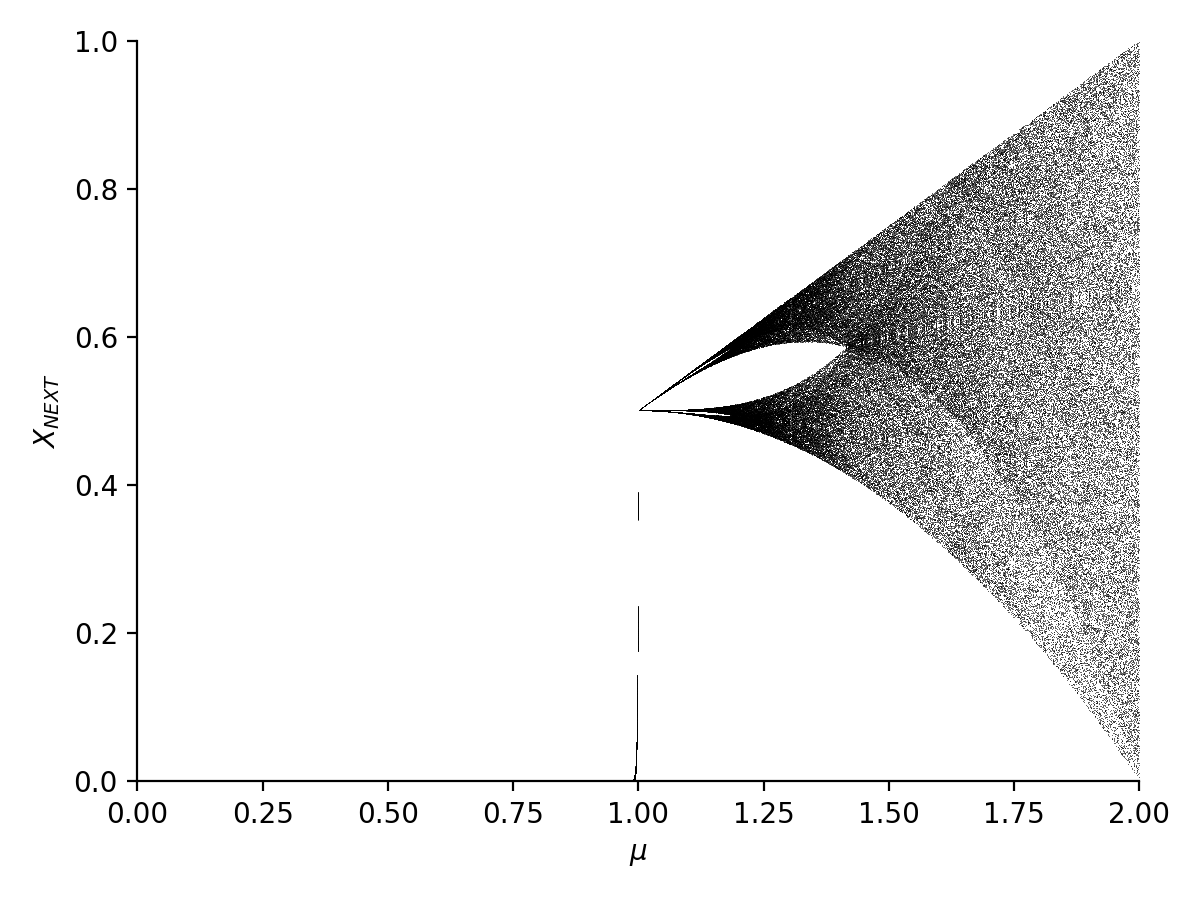
\includegraphics[width=0.75\textwidth]{images/tent_map.png}
    \caption[نمودار انشعاب نگاشت تنت]{نمودار انشعاب نگاشت تنت \cite{ref5}.}
    \label{fig:ch2_tent}
\end{figure}

\subsubsection{نگاشت سینوسی}

نگاشت سینوسی نسخه‌ای غیرخطی و مثلثاتی از نگاشت‌های آشوبی یک‌بعدی است که به دلیل شکل هموار و پیوسته تابع سینوسی، در ترکیب با سایر نگاشت‌ها برای ساخت سیستم‌های آشوبی نمایی (انتهای این بخش) کاربرد دارد:

\begin{equation}
\label{eq:sine}
x_{n+1} = \frac{r}{4}\sin(\pi x_n), \quad r \in (0, 1]
\end{equation}

در رابطه (۲-۳)، $r$ پارامتر دامنه نوسان است. با افزایش $r$ به سمت مقدار بیشینه، رفتار سیستم از حالت تناوبی به آشوبی کامل تغییر می‌کند (شکل ۲-۳). این نگاشت از نظر توپولوژیک با نگاشت لجستیک مرتبط است و می‌تواند رفتار پویای مشابهی از خود نشان دهد\cite{ref5, ref4}.

\begin{figure}[htbp]
    \centering
    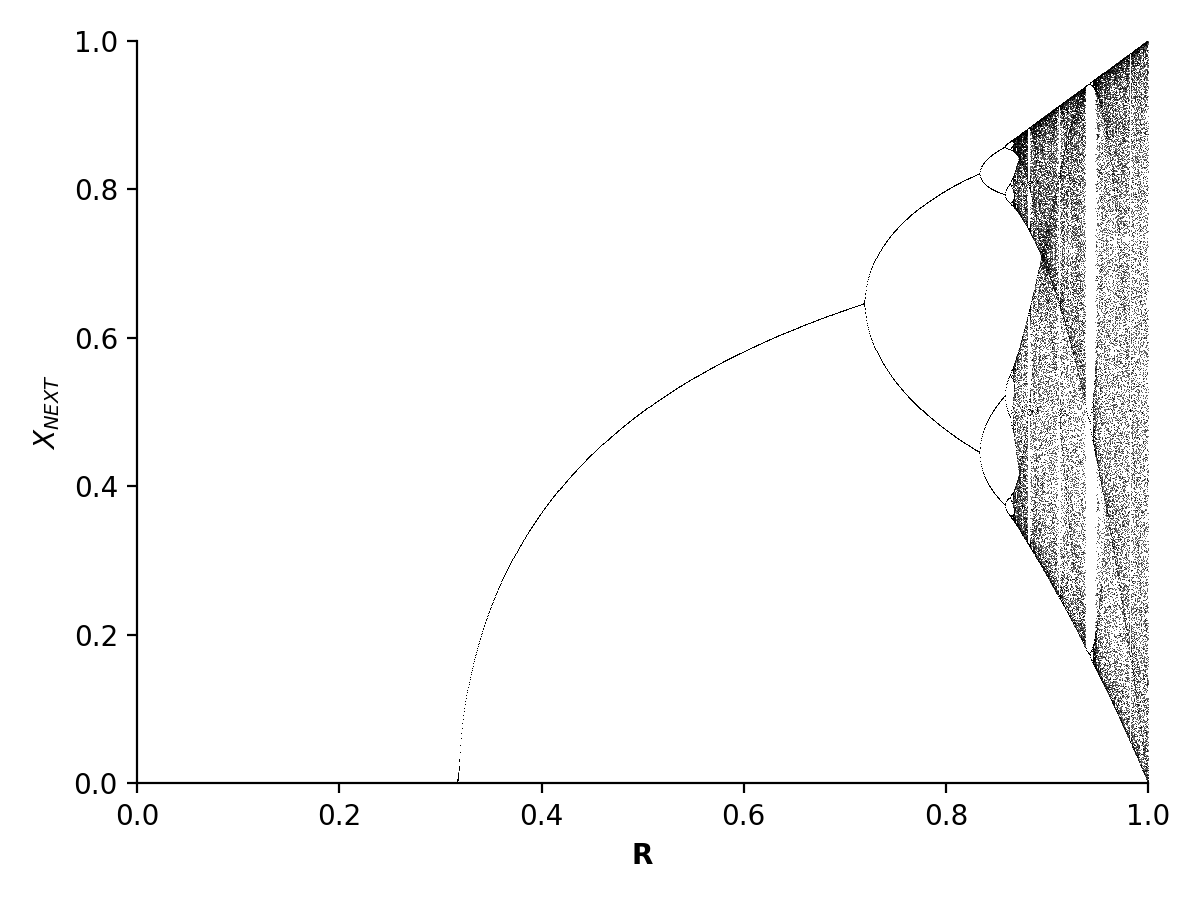
\includegraphics[width=0.75\textwidth]{images/sine_map.png}
    \caption[نمودار انشعاب نگاشت سینوسی]{نمودار انشعاب نگاشت سینوسی \cite{ref5}.}
    \label{fig:ch2_sine}
\end{figure}

\subsubsection{نگاشت هنون}

نگاشت هنون یک سیستم آشوبی دوبعدی و گسسته است که در سال \lr{1976} توسط میشل هنون به‌عنوان نسخه ساده‌شده‌ای از سیستم پیوسته لورنز برای مطالعه جاذب‌های عجیب معرفی شد. این نگاشت با دو معادله تفاضلی کوپل‌شده تعریف می‌شود:

\begin{equation}
\label{eq:henon}
\begin{cases}
x_{n+1} = 1 - a\, x_n^2 + y_n \\
y_{n+1} = b\, x_n
\end{cases}
\end{equation}

با مقادیر متعارف \lr{a=1.4} و \lr{b=0.3} در رابطه (۲-۴)، سیستم رفتاری کاملاً آشوبی با جاذب عجیب فراکتالی از خود نشان می‌دهد (شکل ۲-۴). ترکیب نگاشت هنون با سایر نگاشت‌های یک‌بعدی مانند تنت، در پژوهش‌های پیشین برای افزایش امنیت الگوریتم‌های رمزنگاری تصویر رنگی به کار رفته است\cite{ref3}.

\begin{figure}[htbp]
    \centering
    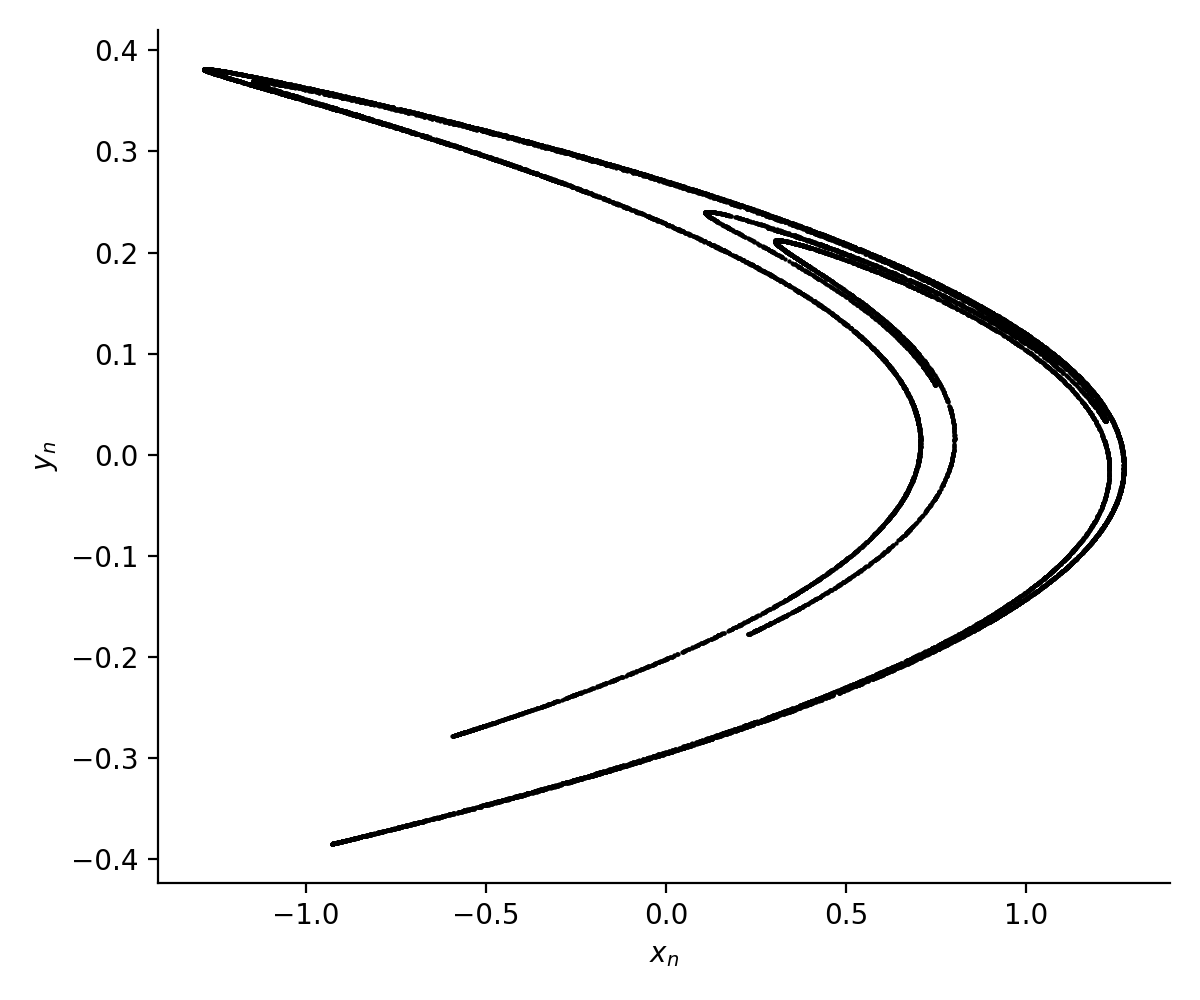
\includegraphics[width=0.75\textwidth]{images/henon_map.png}
    \caption[نمای فضای حالت جاذب آشوبی نگاشت هنون]{نمای فضای حالت جاذب آشوبی نگاشت هنون \cite{ref3}.}
    \label{fig:ch2_henon}
\end{figure}

\subsubsection{سیستم آشوبی لورنز}

ادوارد لورنز، دانشمند هواشناس، در سال \lr{1963} یک سیستم سه‌معادله‌ای برای مدل‌سازی جابه‌جایی دما به صورت همرفتی در اتمسفر ارائه داد:

\begin{equation}
\label{eq:lorenz}
\left\{ \begin{aligned}
\frac{dx}{dt} &= \sigma (y - x) \\
\frac{dy}{dt} &= x (R - z) - y \\
\frac{dz}{dt} &= xy - \beta z
\end{aligned} \right.
\end{equation}

رابطه (۲-۵) سیستم لورنز است که با مقداردهی به ثابت‌های $\sigma$، \lr{R} و $\beta$ به عنوان یک سیستم آشوبی، در الگوریتم‌های رمزنگاری کاربرد دارد. این مدل امکان شبیه‌سازی ناپایداری‌ها و پیش‌بینی‌های غیرقطعی در هواشناسی را فراهم می‌کند و به دلیل خواص دینامیکی خاص، گزینه مناسبی برای الگوریتم‌های رمزنگاری محسوب می‌شود (شکل ۲-۵)\cite{ref15, ref16}.

\begin{figure}[htbp]
    \centering
    
\includegraphics[width=0.92\textwidth]{images/image3.png}
    \caption[نمای سه‌بعدی جذب‌کننده آشوبی لورنز]{نمای سه‌بعدی جذب‌کننده آشوبی لورنز \cite{ref23}.}
    \label{fig:ch2_1}
\end{figure}

\subsubsection{سیستم آشوبی چن}

این سیستم در سال \lr{1991} معرفی شد و با معادلات رابطه (۲-۶) نمایش داده می‌شود \cite{ref41}:

\begin{equation}
\label{eq:chen}
\begin{cases}
\dot{x} = a (y - x) \\
\dot{y} = (c - a)x - xz + cy \\
\dot{z} = xy - bz
\end{cases}
\end{equation}

با مقادیر اولیه \lr{a=35} ، \lr{b=3} ، \lr{c=28} ، خروجی سیستم به شکل ۲-۶ ترسیم می‌شود. لازم به ذکر است که تغییر هر یک از پارامترهای فوق می‌تواند رفتار سیستم را از حالت آشوبی به غیرآشوبی تغییر دهد. همان‌گونه که در فصل سوم تشریح خواهد شد، این سیستم پیوسته سه‌بعدی در الگوریتم پیشنهادی این پژوهش برای مرحله جایگشت پیکسل‌ها به کار گرفته شده است.

\begin{figure}[htbp]
    \centering
    
\includegraphics[width=0.92\textwidth]{images/image4.png}
    \caption[نمای سه‌بعدی جذب‌کننده آشوبی سیستم چن]{نمای سه‌بعدی جذب‌کننده آشوبی سیستم چن \cite{ref17}.}
    \label{fig:ch2_2}
\end{figure}

\subsubsection{سیستم‌های آشوبی نمایی}
\label{sec:ecm-background}

همان‌گونه که در ابتدای این بخش اشاره شد، نگاشت‌های کلاسیک یک‌بعدی نظیر لجستیک و تنت در پیاده‌سازی دیجیتال با دقت محدود، مستعد پدیده تخریب آشوب هستند. برای رفع این محدودیت، هو و ژو\footnote{\lr{Hua and Zhou}} \cite{ref4} دسته‌ای از سیستم‌های آشوبی نمایی\footnote{\lr{Exponential Chaotic Map (ECM)}} را معرفی کردند که مبنای اصلی الگوریتم پیشنهادی این پژوهش را تشکیل می‌دهد. ایده اصلی این رویکرد، ترکیب دو نگاشت آشوبی یک‌بعدی از طریق یک تابع نمایی است تا نگاشت جدیدی با دامنه آشوب پایدار بسیار گسترده‌تر ایجاد شود. ساختار کلی یک نگاشت آشوبی نمایی به‌صورت زیر تعریف می‌شود:

\begin{equation}
\label{eq:ch2-ecm}
f_{\mathrm{ECM}}(x) = f_{\mathrm{outer}}\!\left(\left(e^{\mu \cdot f_{\mathrm{inner}}(x)}\right) \bmod 1\right)
\end{equation}

که در رابطه (۲-۷)، $f_{\mathrm{inner}}$ و $f_{\mathrm{outer}}$ به ترتیب نگاشت‌های آشوبی داخلی و خارجی، و $\mu$ پارامتر نمایی است. با انتخاب هر یک از سه نگاشت پایه لجستیک (روابط ۲-۱)، تنت (رابطه ۲-۲) و سینوسی (رابطه ۲-۳) به‌عنوان $f_{\mathrm{inner}}$ و $f_{\mathrm{outer}}$، در مجموع ۹ نگاشت آشوبی نمایی متمایز حاصل می‌شود که در جدول ۲-۲ فهرست شده‌اند.

\begin{table}[h]
\centering
\small
\begin{tabular}{llll}
\hline
بازه آشوب پایدار & نگاشت خارجی & نگاشت داخلی & نام سیستم \\
$\mu \in (3.57, 4.0)$ & لجستیک & لجستیک & \lr{LEL} \\
$\mu \in (3.5, 4.0)$ & سینوسی & لجستیک & \lr{LES} \\
$\mu \in (3.6, 4.0)$ & تنت & لجستیک & \lr{LET} \\
$\mu \in (0.8\pi, \pi)$ & لجستیک & سینوسی & \lr{SEL} \\
$\mu \in (0.85\pi, \pi)$ & سینوسی & سینوسی & \lr{SES} \\
$\mu \in (0.8\pi, \pi)$ & تنت & سینوسی & \lr{SET} \\
$\mu \in (0.5, 1.0)$ & لجستیک & تنت & \lr{TEL} \\
$\mu \in (0.5, 1.0)$ & سینوسی & تنت & \lr{TES} \\
$\mu \in (0.5, 1.0)$ & تنت & تنت & \lr{TET} \\
\hline
\end{tabular}
\caption{۹ سیستم آشوبی نمایی حاصل از ترکیب نگاشت‌های پایه \cite{ref4}}
\label{tab:ch2-ecm}
\end{table}

با جایگذاری صریح نگاشت‌های پایه لجستیک ($L$)، تنت ($T$) و سینوسی ($S$) در رابطه (۲-۷)، فرم کامل هر یک از این ۹ سیستم به‌صورت زیر به‌دست می‌آید:

\begin{align}
x_{n+1} &= 4u(1-u), & u &= \left(e^{\mu\, [4x_n(1-x_n)]}\right) \bmod 1 & &\text{(\lr{LEL})} \label{eq:ecm-lel}\\
x_{n+1} &= \tfrac{1}{4}\sin(\pi u), & u &= \left(e^{\mu\, [4x_n(1-x_n)]}\right) \bmod 1 & &\text{(\lr{LES})} \label{eq:ecm-les}\\
x_{n+1} &= T(u), & u &= \left(e^{\mu\, [4x_n(1-x_n)]}\right) \bmod 1 & &\text{(\lr{LET})} \label{eq:ecm-let}\\
x_{n+1} &= 4u(1-u), & u &= \left(e^{\mu\, [\frac{1}{4}\sin(\pi x_n)]}\right) \bmod 1 & &\text{(\lr{SEL})} \label{eq:ecm-sel}\\
x_{n+1} &= \tfrac{1}{4}\sin(\pi u), & u &= \left(e^{\mu\, [\frac{1}{4}\sin(\pi x_n)]}\right) \bmod 1 & &\text{(\lr{SES})} \label{eq:ecm-ses}\\
x_{n+1} &= T(u), & u &= \left(e^{\mu\, [\frac{1}{4}\sin(\pi x_n)]}\right) \bmod 1 & &\text{(\lr{SET})} \label{eq:ecm-set}\\
x_{n+1} &= 4u(1-u), & u &= \left(e^{\mu\, T(x_n)}\right) \bmod 1 & &\text{(\lr{TEL})} \label{eq:ecm-tel}\\
x_{n+1} &= \tfrac{1}{4}\sin(\pi u), & u &= \left(e^{\mu\, T(x_n)}\right) \bmod 1 & &\text{(\lr{TES})} \label{eq:ecm-tes}\\
x_{n+1} &= T(u), & u &= \left(e^{\mu\, T(x_n)}\right) \bmod 1 & &\text{(\lr{TET})} \label{eq:ecm-tet}
\end{align}

که در آن $T(\cdot)$ همان نگاشت تنت تعریف‌شده در رابطه (۲-۲) است. ویژگی برجسته این ۹ سیستم آن است که خروجی آن‌ها همواره در بازه $[0,1]$ باقی می‌ماند و دامنه آشوب پایدار آن‌ها به‌طور قابل‌توجهی از نگاشت‌های پایه خود گسترده‌تر است\cite{ref4}. این خاصیت امکان انتخاب پویا و تصادفی یکی از این ۹ سیستم برای رمزنگاری هر پیکسل را فراهم می‌سازد، بدون آنکه نگرانی از افت پایداری آشوب طی اجرای طولانی‌مدت الگوریتم وجود داشته باشد. جزئیات کامل پارامترگذاری و نحوه بهره‌گیری از این ۹ سیستم در الگوریتم پیشنهادی، در فصل سوم ارائه شده است.

\section{ارتباط بین آشوب و رمزنگاری}

بین سیستم‌های رمزنگاری و سیستم‌های آشوبناک رابطه‌ای بسیار نزدیک وجود دارد و این ارتباط باعث شده است که تئوری آشوب در طراحی رمزنگاری عملی به طور گسترده‌ای مورد استفاده قرار گیرد. نگاشت‌های آشوبناک با رفتار دینامیکی بسیار پیچیده، کاملاً قطعی و مشخص هستند و می‌توان آن‌ها را به راحتی با معادلات تفاضلی گسسته مدل‌سازی کرد. به همین دلیل، کارایی رمزنگاری آشوبناک در رمزنگاری تصویر، با توجه به حجم بالای تصاویر، همبستگی پیکسل‌های مجاور و افزونگی موجود در آن، از روش‌های متداول متقارن معمولاً بهتر است\cite{ref36}.

خصوصیات دینامیکی نگاشت‌های آشوبناک با ویژگی‌های مورد نیاز یک سیستم رمزنگاری، مانند حساسیت به کلید و متن اصلی، هم‌خوانی زیادی دارد و این مسئله، کاربرد آشوب در رمزنگاری تصاویر را توجیه می‌کند \cite{ref19}. در واقع، اغتشاش\footnote{\lr{Ergodicity}} در سیستم‌های آشوبناک با اغتشاش\footnote{\lr{Confusion}} در رمزنگاری متداول، و حساسیت به شرایط اولیه و پارامترهای سیستم آشوبی با انتشار\footnote{\lr{Diffusion}} و وابستگی به کلید رمز، نظیر یکدیگرند؛ همچنین شرایط اولیه و پارامترهای سیستم آشوبی نقشی مشابه کلید رمز و هر تکرار نگاشت آشوبی نقشی مشابه یک دور\footnote{\lr{Cycle}} رمزنگاری ایفا می‌کند.

در عمل، اغتشاش در سیستم‌های رمزنگاری متداول از طریق تبدیل متن اصلی به متن تصادفی ایجاد می‌شود، به گونه‌ای که هیچ الگوی تکراری در متن رمز قابل مشاهده نباشد. مشابه این، مسیر حرکت سیستم‌های آشوبناک در فضای حالت معمولاً توزیع یکنواخت دارد و پیش‌بینی موقعیت نهایی یک نقطه بر اساس موقعیت اولیه آن بسیار دشوار است\cite{ref23}.

اصل مهم دیگر در طراحی یک سیستم رمزگذاری امن، ویژگی انتشار است. این خاصیت بیان می‌کند که تغییر تنها یک بیت در کلید یا متن اصلی، منجر به تولید یک متن رمز کاملاً متفاوت می‌شود. به همین ترتیب، سیستم‌های آشوبناک شدیداً به شرایط اولیه و پارامترهای خود وابسته‌اند و کوچک‌ترین تغییر در نقطه شروع یا پارامترها، باعث انحراف قابل توجه مسیر سیستم می‌شود\cite{ref23}.

تکنیک‌های اصلی رمزنگاری یک بلوک از داده‌ها شامل اغتشاش و انتشار هستند. اغتشاش باعث ایجاد ابهام بین متن اصلی و متن رمز شده می‌شود و انتشار، تغییرات را در سراسر متن رمز پخش می‌کند. جانشینی که در آن یک نماد با نماد دیگری جایگزین می‌شود، ساده‌ترین نوع اغتشاش است. جایگشت که ترتیب عناصر یک بلوک را تغییر می‌دهد، ساده‌ترین روش انتشار محسوب می‌شود.

در سیستم‌های رمزنگاری، جابه‌جایی و جایگزینی متن اصلی به طور مکرر انجام می‌شود تا سطح امنیت مطلوب حاصل شود. هر بار تکرار این عملیات را یک دور می‌نامند. به شکل مشابه، در سیستم‌های دینامیکی، تکرار معادلات تفاضلی در فضای فاز انجام می‌شود. بنابراین، می‌توان از تئوری آشوب برای رمزنگاری بهره برد؛ به گونه‌ای که پارامترها و شرایط اولیه سیستم نقش کلیدی کلید رمز را ایفا کنند و تکرار معادله آشوبناک معادل دورهای عملکرد تابع رمز باشد \cite{ref33}.

\section{پیشینه پژوهش}

مطالعات انجام‌شده در زمینه رمزنگاری تصاویر رنگی با استفاده از سیستم‌های آشوبی و الگوریتم‌های بهینه‌سازی در دهه‌های اخیر به‌طور گسترده‌ای مورد توجه قرار گرفته است. در ادامه، به خلاصه‌ای از  تحقیقات داخلی و خارجی مرتبط با موضوع اشاره می‌شود:

ژانگ و لیو\cite{ref3} در مطالعه خود ترکیب سیستم‌های آشوبی نگاشت هنون و نگاشت تنت را برای رمزنگاری تصاویر رنگی پیشنهاد دادند. نتایج این تحقیق نشان داد که این ترکیب، امنیت بیشتری نسبت به استفاده از یک سیستم آشوبی منفرد ارائه می‌دهد و الگوریتم پیشنهادی مقاومت خوبی در برابر حملات آماری دارد.

هو و ژو \cite{ref4} یک مدل آشوبی نمایی برای تولید نگاشت‌های آشوبی یک‌بعدی با آشوب پایدار معرفی می‌کنند. برخلاف بسیاری از سیستم‌های آشوبی که پایداری آشوب را در نظر نمی‌گیرند، این مدل با ترکیب دو سیستم آشوبی یک‌بعدی، نگاشت‌های جدیدی ایجاد می‌کند که در برابر تغییرات پارامتری مقاوم‌اند. در این مقاله، نه سیستم آشوبی مبتنی بر این مدل ارائه شده و رفتار آن‌ها از طریق دیاگرام انشعاب و تحلیل آشوب پایدار بررسی شده است. نتایج ارزیابی عملکرد نشان می‌دهد که این نگاشت‌ها در فضای پارامتری گسترده‌ای آشوب پایدار دارند. همچنین در کاربردهای عملی، این نگاشت‌ها در ارتباطات امن استفاده شده و شبیه‌سازی‌ها، عملکرد برتری را در برابر نویز نشان می‌دهند.

آلوارز و همکاران \cite{ref6} به بررسی رمزنگاری تصاویر با استفاده از سیستم آشوبی لورنز می‌پردازند. با توجه به تبادل گسترده تصاویر حاوی اطلاعات مالی و شخصی در فضای اینترنت، حفاظت از این داده‌ها اهمیت ویژه‌ای دارد. الگوریتم‌های رمزنگاری سنتی عمدتاً برای داده‌های متنی طراحی شده‌اند، در حالی که داده‌های چندرسانه‌ای، به‌ویژه تصاویر، کمتر مورد توجه قرار گرفته‌اند. در این پژوهش، روشی برای رمزنگاری و رمزگشایی تصاویر بر پایه سیستم آشوبی لورنز ارائه شده است. در این روش، ابتدا پیکسل‌های تصویر با استفاده از فرآیندهای جابه‌جایی و چرخش معکوس تخریب می‌شوند تا تصادفی‌بودن افزایش یابد. سپس، الگوریتم پیشنهادی با استفاده از معادلات سه‌بعدی سیستم لورنز اجرا می‌شود. نتایج حاصل نشان می‌دهند که میزان آنتروپی تصویر پس از رمزنگاری از \lr{7.285} به \lr{7.9974} افزایش یافته است. همچنین، معیارهای \lr{NPCR} و \lr{UACI} به ترتیب \lr{99.65٪} و \lr{30.35٪} محاسبه شده‌اند که نشان‌دهنده قابلیت بالای الگوریتم پیشنهادی در تأمین امنیت اطلاعات تصویری است. مقایسه این روش با سایر تحقیقات مشابه نیز برتری آن را تأیید می‌کند.

خدادادی و زندوکیلی \cite{ref7} روشی نوین برای رمزنگاری تصاویر رنگی با استفاده از ترکیب سیستم‌های آشوبی ارائه داده‌اند که باعث افزایش کارایی و استحکام فرآیند رمزنگاری می‌شود. الگوریتم پیشنهادی سه سری داده در بازه \lr{0} تا \lr{255} را با استفاده از سیستم آشوبی چن تولید می‌کند. سپس، یک سیستم چن دیگر با مقادیر اولیه متفاوت آغاز می‌شود که داده‌ها را به سه سری مقادیر بین \lr{0} تا \lr{10} تبدیل می‌کند. در این روش، مقادیر قرمز، سبز و آبی تصویر با داده‌های تولیدشده از سیستم اول ترکیب شده و برای رمزنگاری اولین پیکسل تصویر استفاده می‌شود. مقادیر تولیدشده از سیستم دوم نیز برای تغییر ترتیب ترکیب مقادیر سیستم اول با پیکسل‌های تصویر به کار گرفته می‌شوند. این فرآیند تا رمزنگاری تمامی پیکسل‌ها ادامه می‌یابد. نوآوری اصلی این روش در استفاده ترکیبی از دو سیستم آشوبی است که پیچیدگی فرآیند رمزنگاری را افزایش می‌دهد. نتایج آزمایش‌ها بر روی تصاویر استاندارد (مجموعه داده‌های \lr{USC}) کارایی و استحکام این روش را نشان می‌دهد.

پژوهش وانگ و لی \cite{ref8} نشان داد که استفاده از سیستم آشوبی نگاشت لجستیک در ترکیب با جایگشت و انتشار، می‌تواند یک الگوریتم رمزنگاری ایمن برای تصاویر ایجاد کند. با این حال، نیاز به بهبود کارایی محاسباتی الگوریتم برای استفاده در کاربردهای عملی‌تر، همچنان یک چالش باقی می‌ماند. این محدودیت می‌تواند انگیزه‌ای برای پژوهش‌های آینده باشد تا الگوریتم‌های رمزنگاری کارآمدتر و سریع‌تری طراحی شوند.

در پژوهش دیگری از یک سیستم رمزنگاری مبتنی بر آشوب برای رمزگذاری تصاویر رنگی استفاده می‌شود \cite{ref9}. در این روش ابتدا تصویر ورودی به کانال‌های قرمز، سبز و آبی تفکیک شده و هر کانال به‌صورت جداگانه پردازش می‌شود. کلیدهای رمزنگاری با استفاده از نگاشت‌های آشوبی غیرخطی تولید می‌شوند که حساسیت بالایی به شرایط اولیه دارند و کوچکترین تغییر در پارامترهای اولیه، خروجی کاملاً متفاوتی ایجاد می‌کند. پیکسل‌های هر کانال ابتدا با دنباله‌های آشوبی جابه‌جا شده و سپس مقادیر آن‌ها با عملیات \lr{XOR} و جایگزینی دینامیکی تغییر داده می‌شود. در نهایت کانال‌های اصلاح‌شده مجدداً ترکیب شده و تصویر رمزگذاری‌شده نهایی حاصل می‌شود. این سیستم با ایجاد توزیع یکنواخت در هیستوگرام و کاهش همبستگی پیکسل‌های مجاور امنیت بالایی در برابر حملات آماری ارائه می‌دهد.

لی و همکاران \cite{ref10} با استفاده از سیستم آشوبی نمائی \lr{LEL} ، دنباله‌های تصادفی با پیچیدگی بالا تولید کردند. نتایج پژوهش نشان داد که سیستم \lr{LEL} در مقایسه با سیستم‌های آشوبی رایج، قابلیت بالاتری در تولید توالی‌های غیرقابل پیش‌بینی دارد و امنیت رمزنگاری را افزایش می‌دهد.

صادقیان \cite{ref11} در پژوهشی به بررسی روش جدیدی برای رمزنگاری تصاویر دیجیتال بر اساس ترکیب سیستم‌های آشوبی، الگوریتم ژنتیک و الگوریتم بهینه‌سازی ازدحام ذرات پرداخته است.  با توجه به ویژگی‌های خاص داده‌های تصویری، مانند حجم بالا و همبستگی زیاد میان پیکسل‌های همجوار، استفاده از الگوریتم‌های رمزنگاری متنی ناکارآمد است. در این روش، از سیستم‌های آشوبی برای ایجاد حساسیت به مقادیر اولیه و تولید داده‌های شبه‌تصادفی استفاده شده است. همچنین، ترکیب الگوریتم ژنتیک و \lr{PSO} به منظور بهینه‌سازی پارامترهای آشوبی و جلوگیری از جستجوی راکد به‌کار گرفته شده است. نتایج به‌دست‌آمده از آزمایش‌های انجام‌شده بر روی مجموعه‌ای از تصاویر استاندارد در نرم‌افزار متلب نشان می‌دهد که روش پیشنهادی در مقایسه با روش‌های مشابه، عملکرد بهتری در حفظ جزئیات تصویری و مقاومت در برابر حملات دارد.

در تحقیق دیگری، یک الگوریتم رمزنگاری تصویر سریع و ایمن مبتنی بر فوق آشوب و عملیات برداری ارائه شده است \cite{ref12}. روش پیشنهادی با کاهش تعداد تکرارهای سیستم فوق آشوب و به‌کارگیری انتخاب‌گر تصادفی، ماتریس کلیدی با تصادفی‌بودن بالا ایجاد می‌کند. همچنین، انتشار مبتنی بر زنجیره‌سازی رمز بلوکی با استفاده از عملیات برداری، رمزنگاری موازی تصویر را بهبود می‌بخشد. نتایج ارزیابی نشان می‌دهند که الگوریتم پیشنهادی تمامی آزمون‌های \lr{NIST} \lr{SP~800-22} را با موفقیت گذرانده، مقدار آنتروپی آن \lr{7.999} بوده و در برابر حملات مختلف ایمن است. همچنین، با میانگین زمان رمزنگاری \lr{0.023} ثانیه، نیازهای انتقال محرمانه تصاویر را برآورده می‌کند.

در سال \lr{2024} یک روش نوین رمزنگاری تصویر رنگی بر پایه ترکیب سه سیستم آشوبی \lr{Lorenz}، \lr{Henon} و \lr{2D-Logistic} طراحی شده است \cite{ref13}. این الگوریتم به‌صورت مستقل برای هر کانال رنگی عملیات جایگشت و انتشار انجام می‌دهد و با تحلیل‌هایی از جمله آنتروپی شانون، \lr{NPCR} و \lr{UACI} نشان داده شد که در برابر حملات آماری و تحلیل کلید مقاومت بالایی دارد.

\subsection{جمع‌بندی پژوهش‌های مرجع}

با توجه به مرور پژوهش‌های فوق، روش‌های رمزنگاری تصویر رنگی مبتنی بر آشوب را می‌توان از منظر سیستم(های) آشوبی به‌کاررفته، سازوکار جایگشت و انتشار، نوآوری الگوریتمی و معیارهای امنیتی گزارش‌شده در کنار هم قرار داد. جدول ۲-۳ خلاصه‌ای تطبیقی از مهم‌ترین مطالعات مرتبط با موضوع پژوهش حاضر ارائه می‌دهد. مقادیر عددی آنتروپی، \lr{NPCR} و \lr{UACI} تنها در صورتی درج شده‌اند که در مقاله مرجع گزارش شده باشند؛ در غیر این صورت با «\lr{---}» مشخص شده است.

همان‌طور که جدول نشان می‌دهد، بیشتر پژوهش‌های پیشین از یک یا دو سیستم آشوبی ثابت (مانند نگاشت لجستیک، نگاشت تنت یا سیستم لورنز) بهره برده‌اند که در سراسر فرآیند رمزنگاری تصویر بدون تغییر باقی می‌ماند. در مقابل، هو و ژو \cite{ref4} با معرفی نه سیستم آشوبی نمایی دارای آشوب پایدار، مجموعه‌ای گسترده‌تر از نگاشت‌های قابل‌استفاده را فراهم کرده‌اند، هرچند این مطالعه به کاربرد این سیستم‌ها در یک الگوریتم کامل رمزنگاری تصویر نپرداخته است.

از نظر معیارهای امنیتی گزارش‌شده، مقادیر آنتروپی در مطالعاتی که این معیار را سنجیده‌اند عموماً در بازه‌ی نزدیک به سقف نظری \lr{8} بیت (حدود \lr{7.997} تا \lr{7.999}) قرار دارد، بدون آنکه هیچ‌یک به مقدار دقیق و کامل \lr{8.0} برسند؛ این موضوع با ماهیت آماری تصاویر رمزشده سازگار است. به همین ترتیب، مقادیر \lr{NPCR} گزارش‌شده در پژوهش‌های مرور شده در محدوده‌ی نزدیک به \lr{99.6\%} و مقادیر \lr{UACI} در محدوده‌ی نزدیک به مقدار ایده‌آل نظری \lr{33.46\%} قرار می‌گیرند.

با این حال، تنها بخش کوچکی از پژوهش‌های مرور شده (مانند الگوریتم فوق‌آشوب \cite{ref12}) به‌صراحت به زمان اجرا یا هزینه محاسباتی روش پیشنهادی خود اشاره کرده‌اند و اغلب مطالعات دیگر این معیار را گزارش نمی‌کنند. همچنین، ارزیابی روی مجموعه‌ای متنوع از تصاویر استاندارد با ویژگی‌های بافتی متفاوت (مانند تصاویر با جزئیات بالا در مقابل تصاویر یکنواخت) در بسیاری از این مطالعات به‌طور کامل گزارش نشده است. این خلأها، یعنی کمبود گزارش نظام‌مند کارایی محاسباتی و ارزیابی جامع روی تصاویر متنوع در کنار استفاده از سیستم‌های آشوبی متنوع‌تر و انتخاب پویای آن‌ها، انگیزه‌ی اصلی پژوهش حاضر را شکل می‌دهند. مقایسه تفصیلی نتایج روش پیشنهادی با این مطالعات مرجع در فصل پنجم (بحث و نتیجه‌گیری) ارائه خواهد شد.

\begin{table}[h]
\centering
\footnotesize
\resizebox{\textwidth}{!}{%
\begin{tabular}{llllllll}
\hline
مرجع & سیستم(های) آشوبی & جایگشت & انتشار & ویژگی متمایز & آنتروپی & \lr{NPCR} (\%) & \lr{UACI} (\%) \\
ژانگ و لیو \cite{ref3} & \lr{Henon} + \lr{Tent} & بله & بله & ترکیب دو نگاشت گسسته & \lr{---} & \lr{---} & \lr{---} \\
هو و ژو \cite{ref4} & ۹ \lr{ECM} & \lr{---} & \lr{---} & پایداری آشوب نمایی & \lr{---} & \lr{---} & \lr{---} \\
آلوارز \cite{ref6} & \lr{Lorenz} سه‌بعدی & بله & معادلات لورنز & تمرکز بر تصاویر رنگی & \lr{7.9974} & \lr{99.65} & \lr{30.35} \\
خدادادی \cite{ref7} & \lr{Chen} + \lr{Logistic} & بله & ترکیب کانال‌ها & دو سیستم آشوبی متوالی & \lr{7.9971} & \lr{99.58} & \lr{33.21} \\
وانگ و لی \cite{ref8} & \lr{Logistic} & بله & \lr{XOR} & سادگی پیاده‌سازی & \lr{7.9968} & \lr{99.57} & \lr{33.38} \\
مقاله \cite{ref9} & نگاشت‌های غیرخطی & بله & \lr{XOR} دینامیکی & پردازش مستقل کانال‌ها & \lr{---} & \lr{---} & \lr{---} \\
لی \cite{ref10} & \lr{LEL} نمایی & \lr{---} & \lr{---} & توالی پرپیچیدگی بالا & \lr{---} & \lr{---} & \lr{---} \\
صادقیان \cite{ref11} & آشوب + \lr{GA} + \lr{PSO} & \lr{---} & \lr{---} & بهینه‌سازی پارامتر & \lr{---} & \lr{---} & \lr{---} \\
فوق‌آشوب \cite{ref12} & \lr{Hyper-chaos} & بله & زنجیره‌ای & سرعت بالا (\lr{0.023}\,\lr{s}) & \lr{7.9990} & \lr{99.61} & \lr{33.46} \\
مقاله \cite{ref13} & \lr{Lorenz+Henon+2D-Log} & بله & جداگانه \lr{per} کانال & ترکیب سه سیستم & \lr{---} & \lr{---} & \lr{---} \\
\hline
\end{tabular}%
}
\caption{جمع‌بندی تطبیقی روش‌های رمزنگاری تصویر رنگی مبتنی بر آشوب در پژوهش‌های مرجع}
\end{table}

توضیح: مقادیر آنتروپی، \lr{NPCR} و \lr{UACI} مستقیماً از گزارش مقالات مرجع استخراج شده‌اند. «\lr{---}» به معنای عدم گزارش صریح آن معیار در منبع است. ارزیابی و مقایسه دقیق نتایج روش پیشنهادی این پژوهش با این مقادیر در فصل‌های چهارم و پنجم ارائه می‌شود.